\documentclass[hidelinks]{article}
\usepackage[letterpaper,margin=1.0in]{geometry}
\usepackage[utf8]{inputenc}
\pagenumbering{arabic}
\usepackage{authblk}
\usepackage{graphicx}
\usepackage[singlelinecheck=false]{caption} % singlelinecheck makes single line caption left aligned instead of centered
\usepackage{subcaption}
\usepackage{amsmath}
\usepackage{fancyhdr}
\usepackage{longtable}
\usepackage{booktabs}
% hyperlinks
\usepackage{hyperref}
\usepackage{wrapfig}
\usepackage{xspace}
\usepackage{mathrsfs}
\usepackage{graphicx}
\usepackage{lipsum}
\usepackage{makecell}



\pagestyle{fancy}
\fancyhead[R]{\textbf{\stdpopsim with selection}}

% for highlighting text
\usepackage{xcolor}
\usepackage{soul}

% bibliography
\usepackage[
    backend=biber,
    natbib=true,
    style=authoryear,
    uniquename=false,
    ]{biblatex}
\addbibresource{references.bib}

%\usepackage[round]{natbib}   % omit 'round' option if you prefer square brackets
%\bibliographystyle{plainnat}



\newcommand{\Stdpopsim}{\texttt{Stdpopsim}\xspace}
\newcommand{\stdpopsim}{\texttt{stdpopsim}\xspace}

%commands to format figure and table references in the supplement
\newcommand{\beginsupplement}{%
        \fancyhead[L]{Supplemental Material}
        \setcounter{table}{0}
        \renewcommand{\thetable}{S\arabic{table}}%
        \setcounter{figure}{0}
        \renewcommand{\thefigure}{S\arabic{figure}}%
     }
\newcommand{\stopsupplement}{%
        \setcounter{table}{0}
        \renewcommand{\thetable}{\arabic{table}}%
        \setcounter{figure}{0}
        \renewcommand{\thefigure}{\arabic{figure}}%
     }

\makeatletter
\newcommand{\labelname}[1]{\def\@currentlabelname{#1}}
\makeatother

\newcommand{\tskit}{\texttt{tskit}\xspace}
\newcommand{\slim}{\texttt{SLiM}\xspace}
\newcommand{\msprime}{\texttt{msprime}\xspace}
\newcommand{\snakemake}{\texttt{snakemake}\xspace}

% add commands for msmc2, stairway plot, gone, and smc++
\newcommand{\msmc}{\texttt{msmc2}\xspace}
\newcommand{\stairway}{\texttt{stairwayplot}\xspace}
\newcommand{\gone}{\texttt{GONE}\xspace}
\newcommand{\smcpp}{\texttt{SMC++}\xspace}

% add commands for the DFE inference methods
\newcommand{\dfe}{\texttt{dfe-alpha}\xspace}
\newcommand{\polydfe}{\texttt{polyDFE}\xspace}
\newcommand{\dadicli}{\texttt{dadi-cli}\xspace}
\newcommand{\grapes}{\texttt{GRAPES}\xspace}

% add commands for the sweep detection methods
\newcommand{\sweepfinder}{\texttt{sweepfinder2}\xspace}
\newcommand{\diploshic}{\texttt{diploshic}\xspace}

% Avoid pandoc bug when there are lists in the body.
\providecommand{\tightlist}{%
\setlength{\itemsep}{0pt}\setlength{\parskip}{0pt}}

\newcommand{\rngcomment}[1]{\textcolor{red}{RNG: #1}}

\newcommand{\kelcomment}[1]{\textcolor{blue}{KEL: #1}}

\newcommand{\drscomment}[1]{\textcolor{purple}{DRS: #1}}

\newcommand{\igcomment}[1]{\textcolor{orange}{IG: #1}}

\title{Accessible, realistic genome simulation with selection using \stdpopsim}

% author tranche explanation:
% co-first authors
\author[1,*]{Graham Gower}
\author[2,*]{Nathaniel S. Pope}
\author[2,3,*]{Murillo F. Rodrigues}
\author[2,*]{Silas Tittes}
\author[4,*]{Linh N. Tran}

% additional authors
\author[5]{Ornob Alam}
\author[6]{Maria Izabel A. Cavassim}
\author[7]{Peter D. Fields}
\author[8]{Benjamin C. Haller}
\author[9,10]{Xin Huang}
\author[11]{Ben Jeffrey}
\author[2]{Kevin Korfmann}
\author[6]{Christopher C. Kyriazis}
\author[2]{Jiseon Min}
\author[12]{Inés Rebollo}
\author[2]{Clara T. Rehmann}
\author[2]{Scott T. Small}
\author[2]{Chris C. R. Smith}
\author[13]{Georgia Tsambos}
\author[11]{Yan Wong}
\author[14]{Yu Zhang}

% PI additional authors
\author[15]{Christian D. Huber}
\author[14]{Gregor Gorjanc}
\author[16]{Aaron P. Ragsdale}

% PIs that were very involved in the project
\author[17]{Ilan Gronau}
\author[4]{Ryan N. Gutenkunst}
\author[11]{Jerome Kelleher}
\author[6]{Kirk E. Lohmueller}
\author[18]{Daniel R. Schrider}
\author[2,19]{Peter L. Ralph}
\author[2,$\heartsuit$]{Andrew D. Kern}

\affil[*]{\small{These authors contributed equally to the paper.}}
\affil[$\heartsuit$]{\small{To whom correspondence should be addressed.}} 
\affil[1]{\small{Section for Molecular Ecology and Evolution, Globe Institute, University of Copenhagen, Denmark}}
\affil[2]{\small{Institute of Ecology and Evolution, University of Oregon, Eugene, OR, 97402, USA}}
\affil[3]{\small{Division of Genetics, Oregon National Primate Center, Oregon Health and Science University, Beaverton, OR, 97006, USA}}
\affil[4]{\small{Department of Molecular and Cellular Biology, University of Arizona, Tucson, AZ, 85721, USA}}
\affil[5]{\small{Center for Genomics \& Systems Biology, New York University, New York, NY, 10003, USA}}
\affil[6]{\small{Department of Ecology and Evolutionary Biology, University of California, Los Angeles, Los Angeles, CA, USA}}
\affil[7]{\small{The Jackson Laboratory, Bar Harbor, ME, 04609, USA}}
\affil[8]{\small{Department of Computational Biology, Cornell University, Ithaca, NY, USA}}
\affil[9]{\small{Department of Evolutionary Anthropology, University of Vienna, Vienna, Austria}}
\affil[10]{\small{Human Evolution and Archaeological Sciences (HEAS), University of Vienna, Vienna, Austria}}
\affil[11]{\small{Big Data Institute, Li Ka Shing Centre for Health Information and Discovery, University of Oxford, Oxford OX3 7LF, UK}}
\affil[12]{\small{Instituto Nacional de Investigación Agropecuaria (INIA), Estación Experimental Las Brujas, Ruta 48 km 10, Canelones, Uruguay}}
\affil[13]{\small{Department of Genome Sciences, University of Washington, Seattle, WA, 98195, USA}}
\affil[14]{\small{The Roslin Institute and Royal (Dick) School of Veterinary Studies, University of Edinburgh, Edinburgh EH25 9RG, UK}}
\affil[15]{\small{Department of Biology, Pennsylvania State University, University Park, PA, 16802, USA}}
\affil[16]{\small{Department of Integrative Biology, University of Wisconsin-Madison, Madison, WI, USA}}
\affil[17]{\small{Efi Arazi School of Computer Science, Reichman University, Herzliya 4610101, Israel}}
\affil[18]{\small{Department of Genetics, University of North Carolina at Chapel Hill, Chapel Hill, NC, 27599, USA}}
\affil[19]{\small{Department of Data Science, University of Oregon, Eugene, OR, 97402, USA}}


\date{\small{\today{}}}

\begin{document}

\maketitle


\section*{Abstract}
    \label{abstract}
    Selection is a fundamental evolutionary force that shapes patterns of genetic variation across species.
    However, simulations incorporating realistic selection along heterogeneous genomes in complex demographic histories
    is challenging, limiting our ability to benchmark statistical methods aimed at detecting selection and to explore theoretical predictions.
    \stdpopsim is a community-maintained simulation library that already provides an extensive catalog of
    species-specific population genetic models.
    Here we present a major extension to the \stdpopsim{} framework that enables simulation of various modes
    of selection, including background selection, selective sweeps,
    and arbitrary distributions of fitness effects (DFE) acting on annotated subsets of the genome (for instance, exons).
    This extension maintains \stdpopsim's core principles of reproducibility and accessibility while adding support
    for species-specific genomic annotations and published DFE estimates.
    We demonstrate the utility of this framework by benchmarking methods for demographic inference,
    DFE estimation, and selective sweep detection across several species and scenarios.
    Our results demonstrate the robustness of demographic inference methods to selection on linked sites,
    reveal the sensitivity of DFE-inference methods to model assumptions,
    and show how genomic features, like recombination rate and the density of functional sequence, influence power to detect selective sweeps.
    This extension to \stdpopsim{} provides a powerful, new resource for the population genetics community
    to explore the interplay between selection and other evolutionary forces in a reproducible, low-barrier framework.

\section*{Introduction}
    \label{introduction}
    % selection
    Selection is a fundamental force in evolution, shaping the
    genetic diversity of populations and driving the adaptation of
    species to their environments. The effects of selection
    on genetic variation are complex, and can be difficult to disentangle
    from other evolutionary processes such as mutation, recombination,
    and genetic drift \citep[e.g.,][]{gillespie1991causes}.
    For instance, changes in population size can lead to fluctuations
    in genetic diversity across a recombining chromosome
    that can mimic the effects of selection \citep{simonsen1995properties},
    and lead to spurious inferences about the strength and targets of genetic adaptation
    \citep{simonsen1995properties,akey2004population,nielsen2005genomic}.
    In turn, selection can confound our ability to infer demographic
    history from allele frequencies \citep{ewing2016consequences,schrider2016effects} and
    estimates of inverse coalescent rate \citep{schrider2016effects, johri2021impact, cousins2024accurate}.
    Thus, it is imperative to jointly account for the effects of selection
    and demography when inferring evolutionary history from genetic data \citep[e.g.,][]{sheehan2016deep,johri2020toward},
    yet the number of tools for doing so remain limited.

    % simulation
    To meet the growing need for the interpretation,
    analysis, and exploration of realistic and complex evolutionary models,
    the field of population genetics has increasingly turned to simulation.
    Simulation in population genetics has a long history
    including both backward-in-time coalescent simulations
    \citep{kingman1982genealogy,hudson1983testing, hudson1990gene}
    and forward-in-time simulations of complex demography and selection
    \citep[e.g.,][]{gillespie1984molecular, hernandez2008flexible, thornton2014c++, haller2019slim, gaynor2021AlphaSimR}.
    The development of simulation tools has been driven by the need to
    understand the effects of complex evolutionary processes on genetic
    variation \citep[e.g.,][]{peischl2013accumulation, thornton2019polygenic, galloway2020few, zhang2020impact},
     to provide a null model for hypothesis testing
    \citep[e.g.,][]{hudson1992statistical,hudson1994evidence,sabeti2002detecting},
    to explore the power and limitations of statistical methods \citep[e.g.,][]{przeworski2002signature, macleod2014effects},
    and increasingly to provide a basis for machine learning and other
    simulation-based inference methods
    \citep[e.g.,][]{beaumont2002approximate,lin2011distinguishing,kern2018diplos,mughal2019localizing,sanchez2021deep,wang2021automatic, zhang2023maladapt, smith2023dispersenn2}.
    However, joint simulation of complex demography and selection on realistic genomes is challenging,
    requiring many choices including the strength and rate of selection,
    and a parameterized demographic model,
    as well as implementation of genetic maps and other genomic features related to the strength of selection.
    This is a daunting task, and can be a barrier to
    the adoption of simulation-based methods in population genetics.
    Furthermore, different simulation and inference tools may use different structures
    and parameter scalings for their models,
    making it difficult to directly compare across these tools and the studies that use them.

    % stdpopsim
    In light of the complexities associated with estimating and simulating
    population genetic models, it is no surprise that
    a lingering challenge with simulation in population genetics has been
    reproducibility and the ability to share and compare results among
    researchers \citep[e.g.,][]{ragsdale2020lessons}.
    This challenge has been addressed in part by the development
    of community resources for sharing and distributing simulation software
    via the \stdpopsim project \citep{adrion2020community}. \stdpopsim
    provides a standardized interface for accessing a wide range of
    population genetic models, and has been widely adopted by the community
    \citep[e.g.,][]{speidel2021inferring, wang2021automatic, yang2022trustgwas, degiorgio2022spatially, browning2023fast, schweiger2023ultrafast, temple2024modeling, haag2025pandora}.
    Yet, previous releases of \stdpopsim did not include
    models of selection, which is a major limitation for more empirically motivated
    applications of population genetic simulation. In particular, modeling selection
    through simulation is critical for understanding processes such
    as adaptation \citep[e.g.][]{thornton2019polygenic,hartfield2024polygenic}, the effects of selective sweeps
    \citep[e.g.][]{braverman1995hitchhiking,fay2000hitchhiking,przeworski2002signature,przeworski2005signature,schrider2015soft},
    and the impact of background selection on genetic diversity
    \citep[e.g.][]{charlesworth1993effect,charlesworth1995pattern,williamson2002genealogy,ewing2016consequences,torres2020temporal}.
    Ideally, one would like
    to have a simple, unified framework for simulating both neutral and
    non-neutral evolutionary processes and to be able to compare the
    results of these simulations to empirical data in a manner that is
    both accessible to a wide range of researchers and highly reproducible.
    Furthermore, the framework should include the complex realities of
    genomes, including heterogeneous recombination rates,
    variation in the size and density of functional elements, and
    non-equilibrium demographic histories. Moreover, one should be able
    to model all of these features simultaneously using estimates and annotations obtained
    from a species of interest \citep[e.g.][]{schrider2020background,rodrigues2024shared}.
    %
    \stdpopsim{} provides a framework for such models,
    thus lowering the barrier to production of complex, multifaceted simulations,
    and allowing a wider range of researchers to make use of high-quality simulations
    in developing or testing their work.
    The project also holds as a central goal open, collaborative, and inclusive work,
    viewing capacity-building across the community as equal in importance to software development.

    % goals
    Here, we provide an overview of a major new addition
    to \stdpopsim---the inclusion of models of selection.
    We begin by describing the models of selection that we have implemented,
    as well as the parameter choices that are available to the user.
    This includes models of background selection, selective sweeps, and
    models of the distribution of fitness effects (DFE).
    Further, we describe how these can be applied not only genome-wide but to
    genomic regions with a particular annotation, specific to a given species available
    through the \stdpopsim API, and combined with a parameterized model of
    demography and recombination to provide a realistic simulation of
    genetic variation in a population.
    We then provide a series of examples of how these models can be used
    to benchmark and compare the performance of different methods for
    using genetic data to infer demographic history, the distribution of fitness effects,
    and the targets of recent positive selection.

\section*{Implementing Selection in \stdpopsim}
    \label{selection}

    % implementing selection
    \stdpopsim previously provided a wide range of models of neutral
    demographic history from roughly two dozen species \citep{lauterbur2023expanding}.
    This was accomplished through the use of a standardized interface
    and data structure that allows for the curated addition of new
    species and models, and can use either
    \msprime \citep{Baumdicker2022} or \slim \citep{haller2019slim}
    as the backend engine for efficient population genetic simulation.
    To extend \stdpopsim's functionality to include models of selection,
    we introduce two new classes
    to the \stdpopsim API: the \texttt{DFE} class and the \texttt{Annotation} class.
    The \texttt{DFE} class provides an interface for specifying
    a distribution of the fitness effects (DFE) of new mutations.
    Each \texttt{DFE} object specifies a list of mutation types and
    their proportions, where
    each mutation type is associated with a dominance coefficient,
    (currently limited to values between 0 and 1, inclusive),
    the distribution of selection coefficients (e.g., fixed-value, normally-distributed, gamma-distributed),
    and the parameters of this distribution.
    Each \texttt{Annotation} object represents a collection of functional
    genomic elements (e.g., exons, introns, intergenic regions, etc.)
    whose coordinates are specified using a GFF3 annotation file.
    More concretely, consider implementing a model of selection consistent with the
    DFE inferred by Kim et al. (\citeyear{kim2017inference}) for exons in the human genome.
    The associated \texttt{DFE} object is defined with two mutation types,
    neutral and deleterious, corresponding to synonymous and non-synonymous sites,
    with their proportions set to their expected prevalence in exons.
    The neutral mutation type is associated with a fixed selection coefficient (0),
    and the deleterious mutation type is associated with a dominance coefficient of $0.5$ and
    a gamma-distributed selection coefficient
    with mean and shape as inferred by Kim et al. (\citeyear{kim2017inference}).
    \texttt{DFE} objects can also model a relationship between the selection and dominance coefficients \citep{huber2018gene}
    by defining ranges of selection coefficients and associating each range with a different dominance coefficient (see below).


    \begin{figure}[t!]
        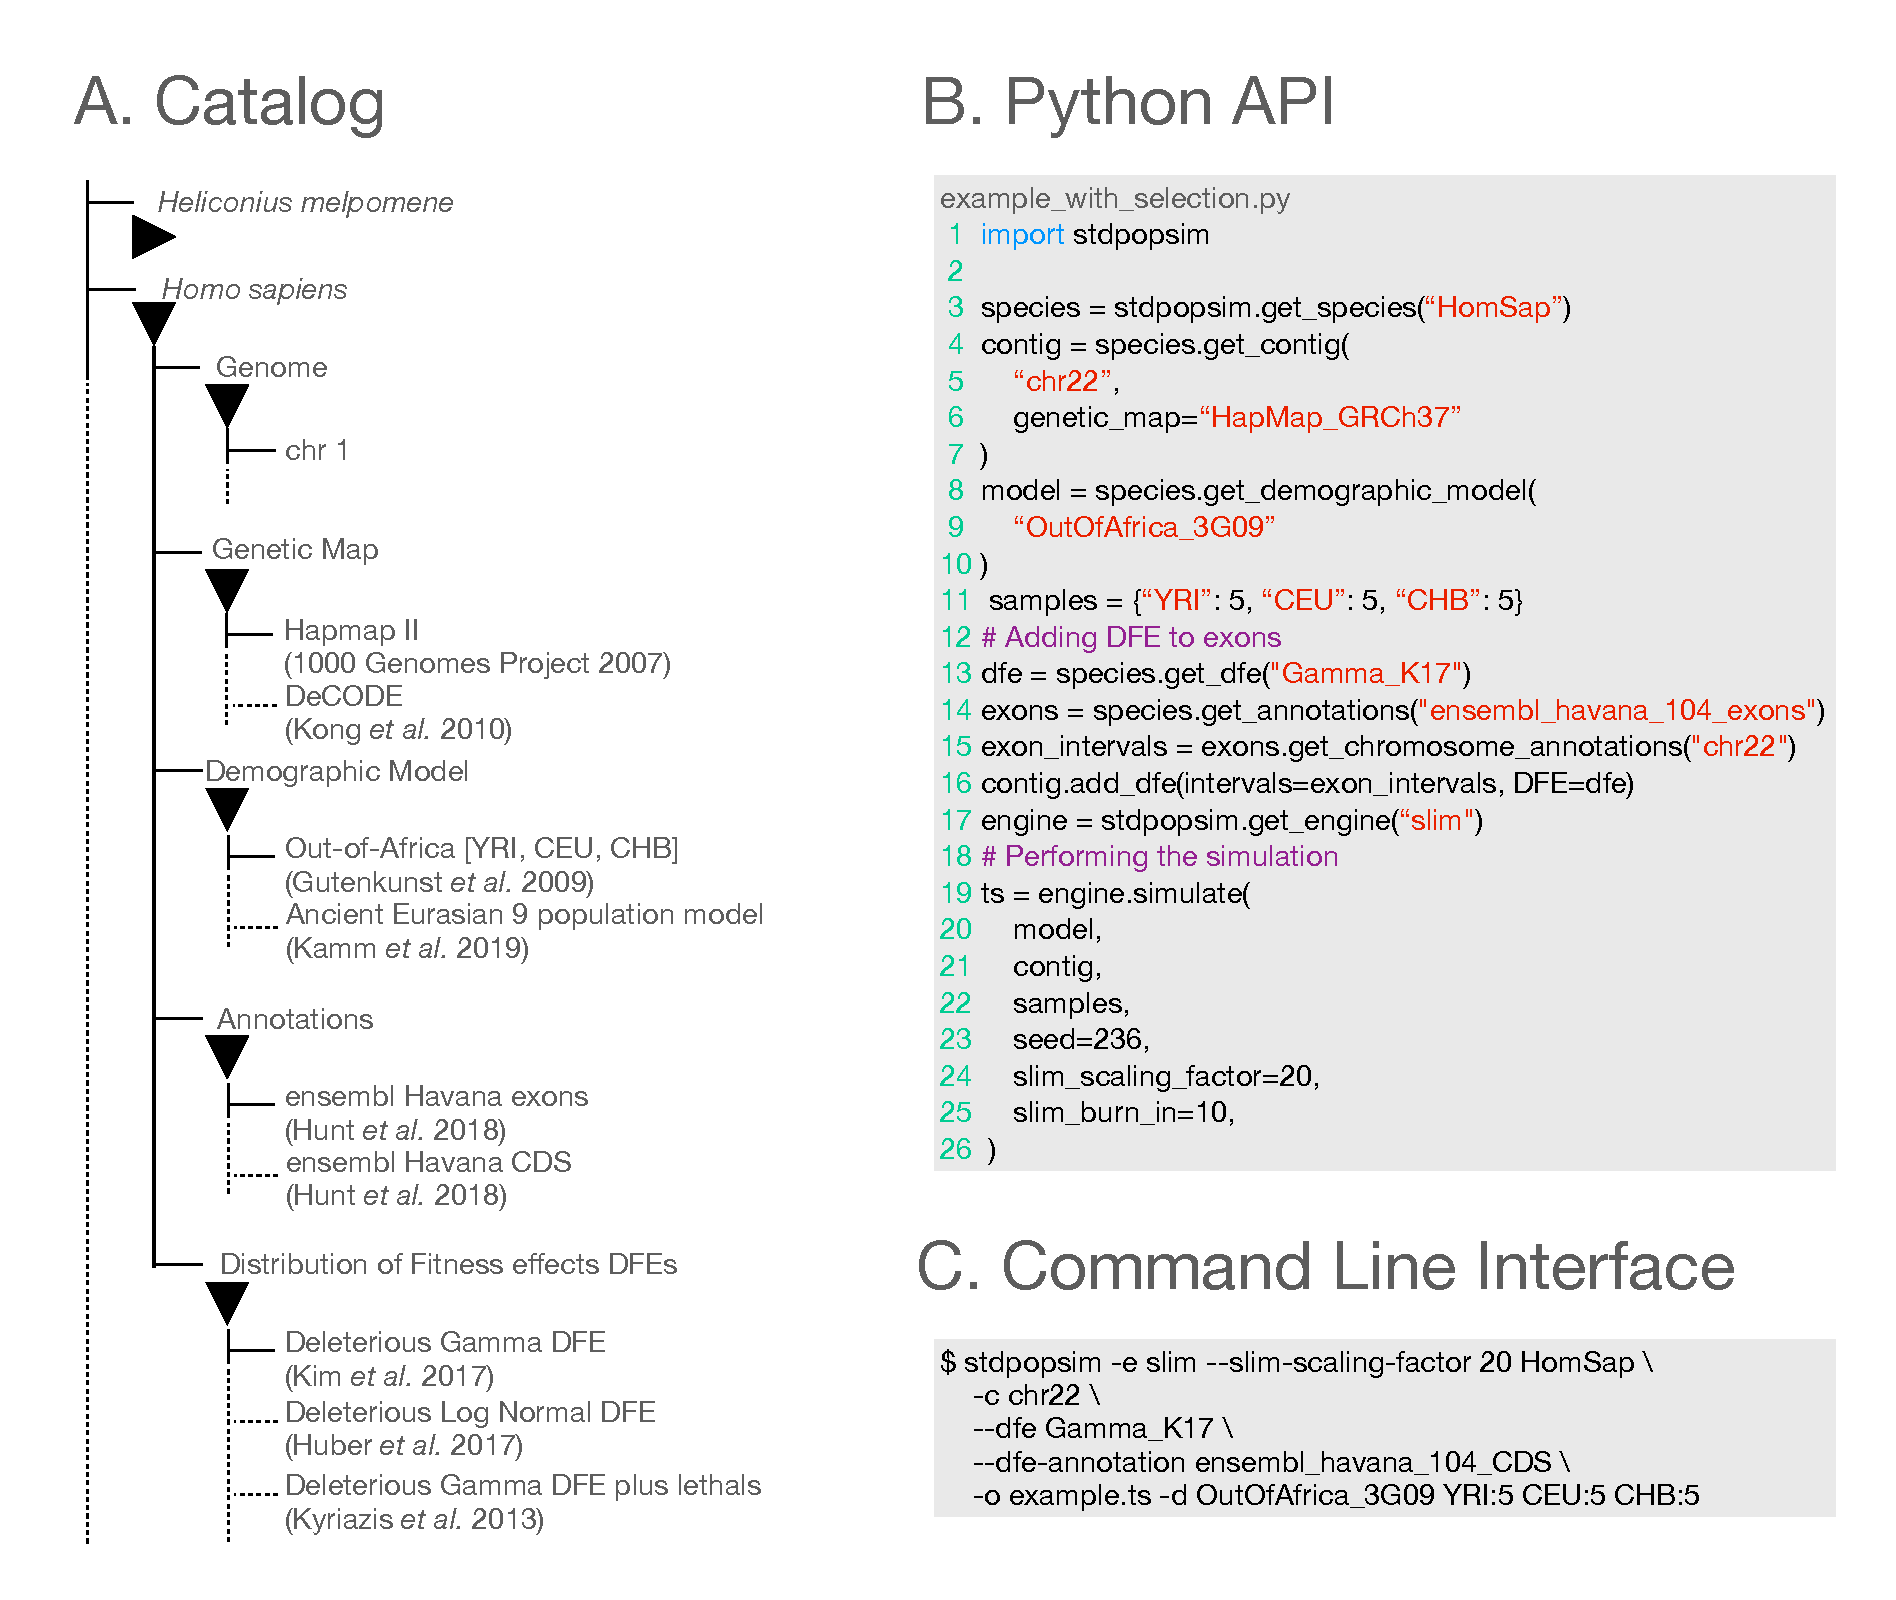
\includegraphics[width=\linewidth]{figures/schematics/catalog.pdf}
        \caption{\label{fig:schematic}
        \textbf{(A)} A schematic of the \stdpopsim catalog and the different components that
        can be used in simulations.
        \textbf{(B)} The python API and \textbf{(C)} the command line interface.
        The user specifies a species, a portion of
        the genome to simulate, and optionally a genetic map, a model of
        demography, and a model of selection that itself is composed of a
        distribution of fitness effects (DFE) and a set of functional
        annotations. }
    \end{figure}

    As with other aspects of \stdpopsim, we intend the selection models to be as biologically accurate as possible.
    Thus, the \stdpopsim catalog provides \texttt{Annotation} objects based on species' publicly available functional genomic elements
    and \texttt{DFE} objects based on published DFE estimates (Figure \ref{fig:schematic}A).
    By using annotation objects, one can, for example, simulate populations where selected mutations (whose selection
    coefficients are drawn from a specified DFE) occur within annotation regions (e.g. exons), while all mutations
    occurring outside of these regions do not affect fitness.
    There are relatively few species with published DFE estimates in the literature.
    \stdpopsim currently has implemented DFEs for five species in the catalog:
    \textit{Arabidopsis thaliana} \citep{huber2018gene},
    \textit{Drosophila melanogaster} \citep{ragsdale2016triallelic,huber2017determining,zhen2021greater},
    humans \citep{huber2017determining,kim2017inference,kyriazis2022using,castellano2019compmarison,castellano2019compmarison,rodrigues2024shared},
    \textit{Mus musculus} \citep{booker2021selective},
    and the vaquita porpoise \textit{Phocoena sinus} \citep{robinson2022critically}.
    While the DFEs are from a limited number of species, these DFEs can be applied to other species
    in the catalog if and when it is suitable.
    For instance, one could simulate a butterfly species with a gamma-distributed DFE originally
    estimated from humans, or a human population with a DFE estimated from \textit{Drosophila}.
    Indeed, the DFE labeled \texttt{HomSap/Mixed\_K23} is recommended by \citet{kyriazis2022using}
    for ``general'' use across species (lacking more specific information).
    Furthermore, the user can specify a custom DFE and provide their own annotations
    of functional elements to simulate selection in a species for which we do not yet have
    a published DFE included in the catalog.

    From a user's perspective, a model of selection is specified by pairing a \texttt{DFE} object
    with a collection of genomic segments defined using an \texttt{Annotation} object.
    Multiple such pairings can be defined in one simulation
    to provide a rich model of how selection may vary along a chromosome.
    For example, coding sequences may be associated with one DFE and non-coding sequences in exons with another DFE.
    Simulations with selection are then implemented by specifying a species,
    a portion of the genome to simulate,
    a genetic map if available, a model of demography, and pairings of DFEs with genomic segments
    using either the python API or the command-line interface (Figure \ref{fig:schematic}B-C).
    Simulations with selection are generated
    using the \slim simulation engine, which is perhaps
    the most flexible simulation engine for modeling selection available to date
    (\msprime's selection models are relatively limited and thus not currently used by \stdpopsim).

    % sweep interface
    In addition to the \texttt{DFE} class, we have also implemented a class (\texttt{stdpopsim.selective\_sweep})
    that enables selective sweeps to be simulated in \stdpopsim.
    This class augments a demographic model with an event
    which conditions on the introduction of a selected mutation at a given time and position
    and with a given selection coefficient. Further, the user can specify the minimum frequency
    of the selected allele at the time of sampling. As this functionality is implemented
    on top of the existing \stdpopsim API, it can be combined with other models of selection
    and demography to provide a model of the combined effects of multiple, disparate evolutionary processes
    on genetic variation in a population.


    % current numbers of DFEs / species / etc
    At this release (version 0.3.0) the \stdpopsim catalog comprises 27 species (i.e. genome representations)
    for which we have included 35 demographic models, 38 genetic maps, 12 DFEs, and 8 annotation objects. %ADK: checked this on 3/10/25
    Additions to the catalog are ongoing---we point the reader to our previously published
    report detailing this effort \citep{lauterbur2023expanding}. We welcome contributions from the
    community and encourage those interested in contributing to visit \url{https://popsim-consortium.github.io/stdpopsim-docs}
    or contact one of the PopSim Consortium members for guidance.



    \section*{Inference of $N_e(t)$ in the context of selection}
    One of the most common applications of population genetic inference is to estimate
    the effective population size over time, $N_e(t)$, from genetic data. This can be done
    using a variety of methods, including the sequential Markovian coalescent
    \citep{li2011inference,Schiffels2020,terhorst2017robust},
    through use of the site frequency spectrum (SFS) \citep{liu2020stairway},
    as well as through identity by descent information \citep{santiago2020recent}.
    Since all of these methods assume neutrality, they are typically applied to genomic
    segments that are not expected to be directly affected by selection (e.g., by masking exons
    and conserved elements).
    However, selection acting on linked sites---even those that are masked out of the
    analysis---can bias estimates of $N_e(t)$
    away from census population sizes by increasing the
    rate of coalescence in the genome \citep[e.g.][]{schrider2016effects}.
    Using \stdpopsim, we can readily examine how different methods for inferring $N_e(t)$
    are influenced by selection on linked sites,
    which in the case of negative selection is commonly referred to as \emph{background selection}
    \citep{charlesworth1993effect,hudson1995deleterious}.


    \begin{figure}[b!]
        \centering
        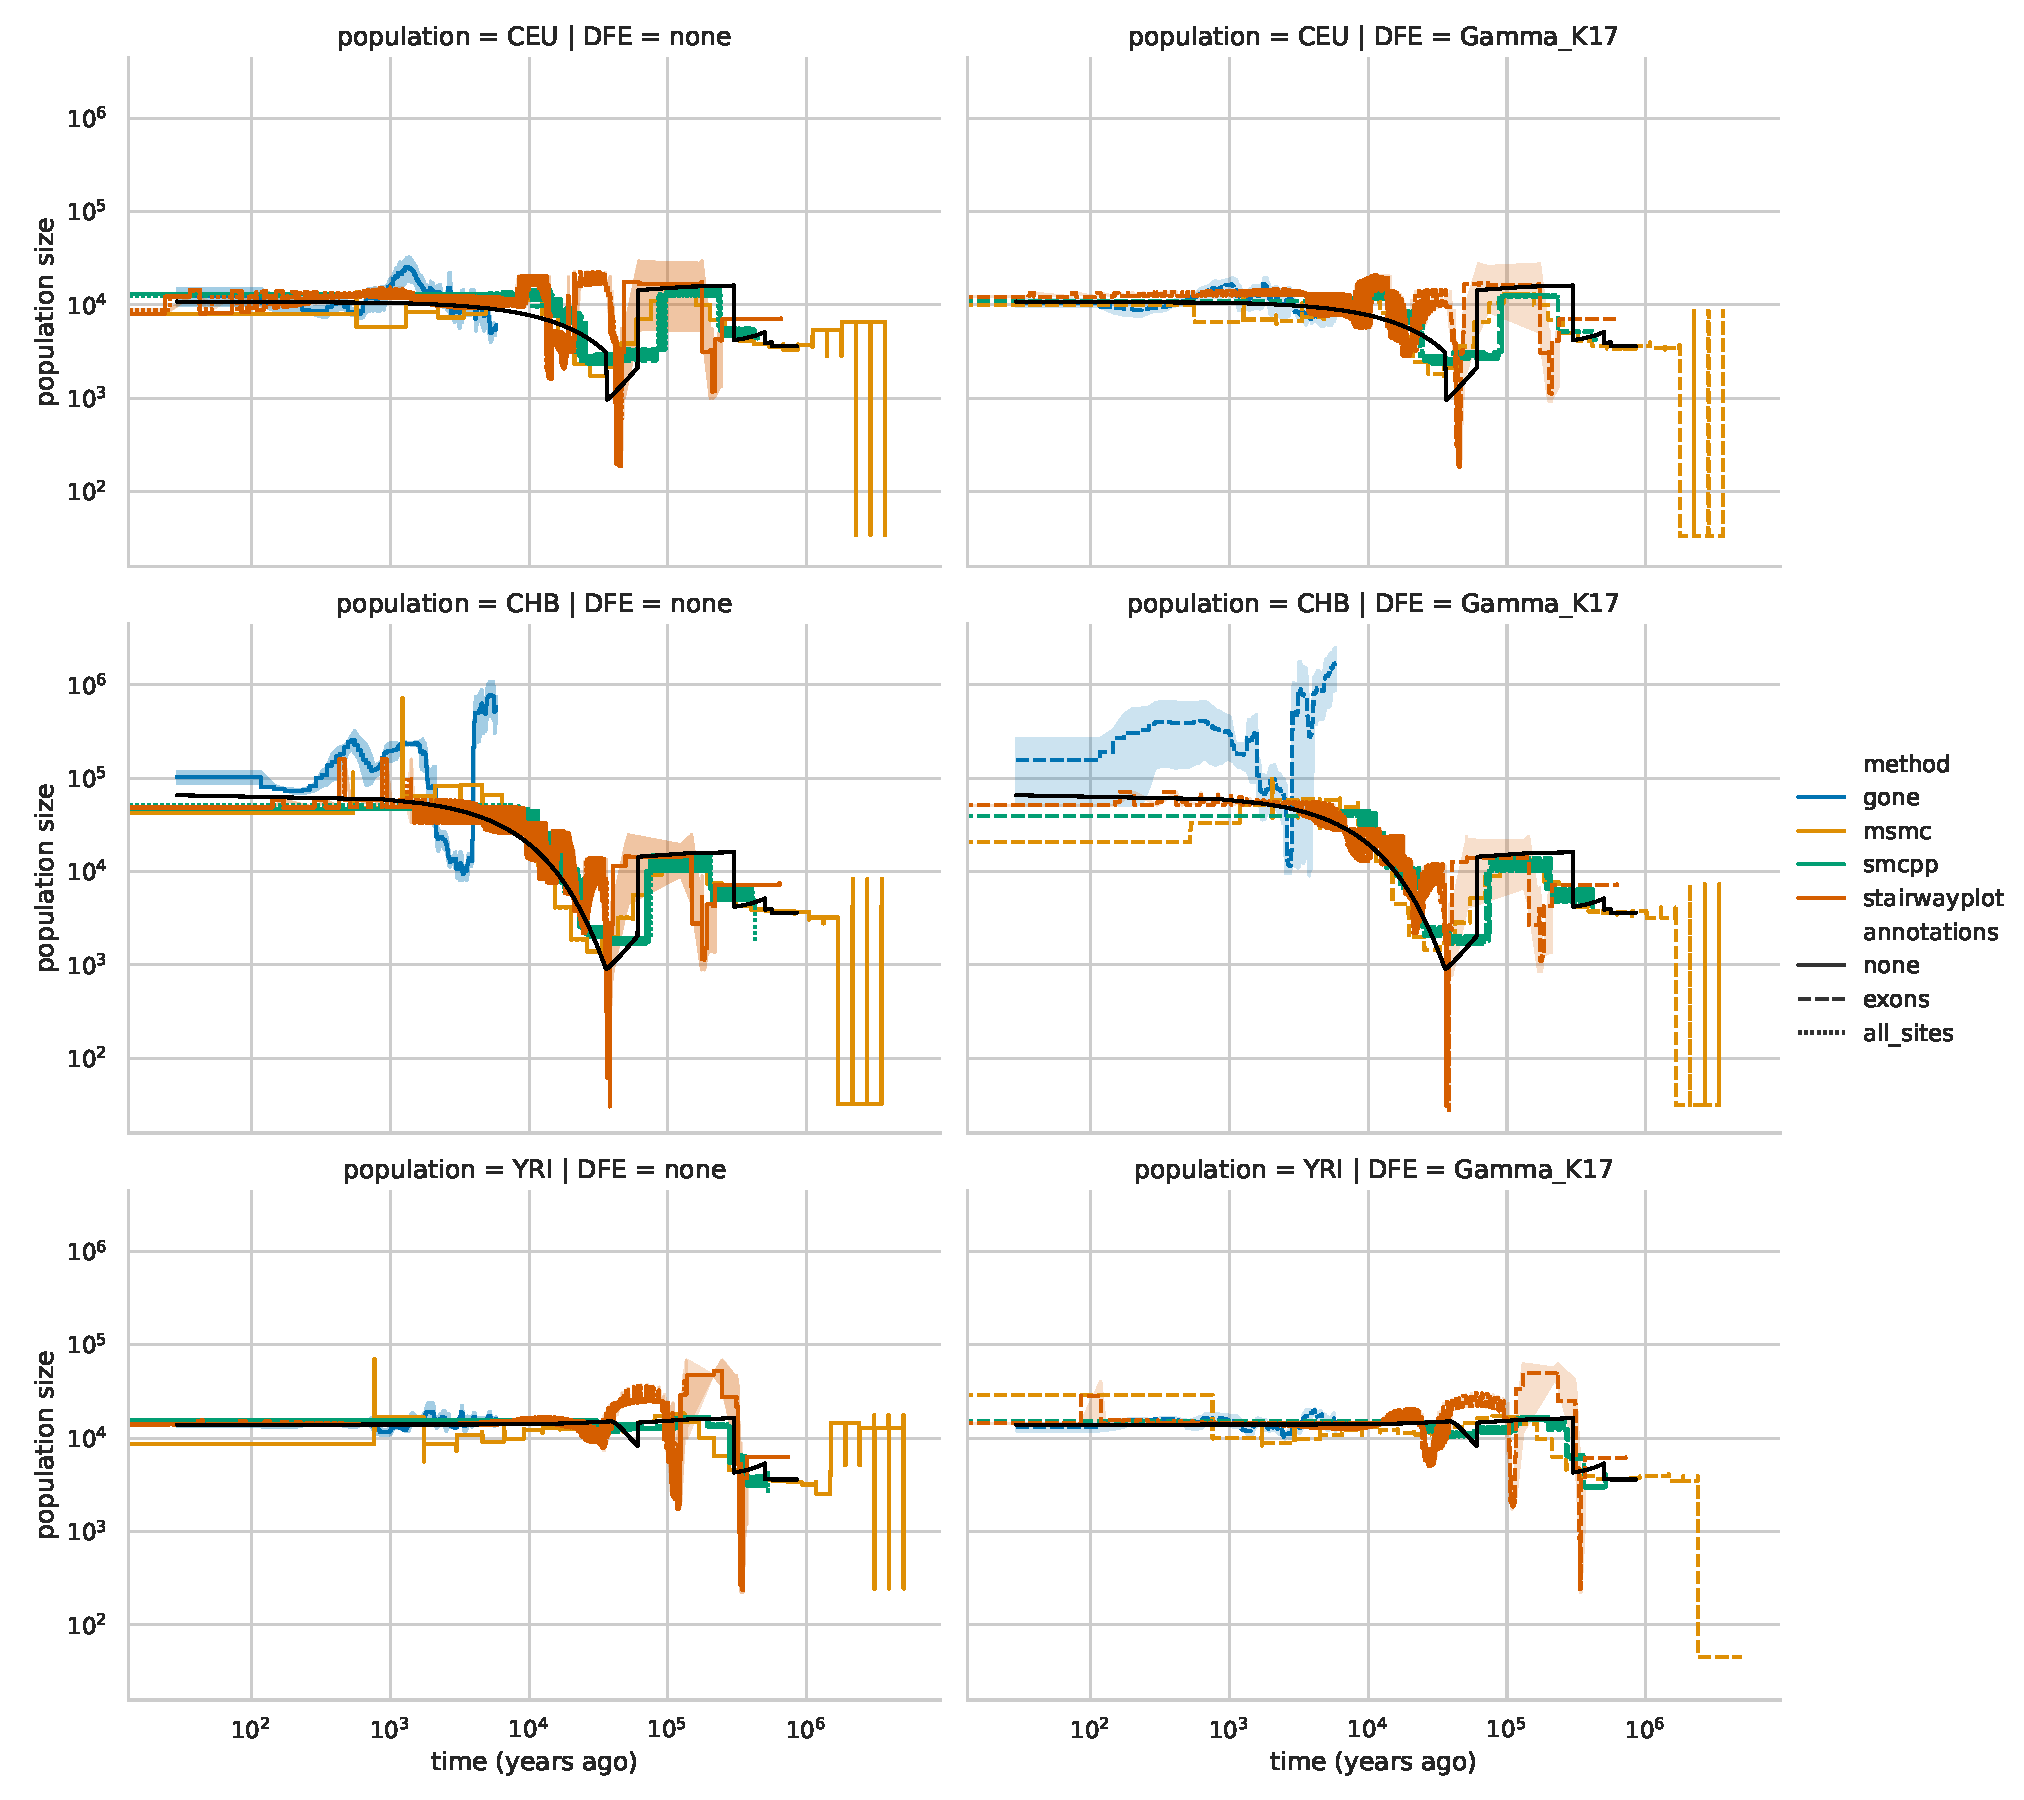
\includegraphics[width=\textwidth]{figures/HomSap/OOA/estimated_Ne_t_final}
        \caption{
        \label{fig:human-demography}
        %citations aren't always allowed in captions. We should check with MBE.
        %IG:I removed citations from all fig captions. They are prominently specified in the main text
        Inference of $N_e(t)$ from human genomes simulated under an out-of-Africa demographic model
        with and without purifying selection on exons.
        Rows correspond to the three extant populations in the simulation: CHB, CEU, and YRI.
        Columns correspond to the four inference methods:
        \stairway, \msmc, \smcpp and \gone.
        Each plot depicts the inferred $N_e(t)$ on the three datasets simulated without selection (blue)
        and the three datasets simulated with the background effects of purifying selection on exons (orange),
        alongside the true values of $N_e$ used in simulation (black).
        }
    \end{figure}

    To do this we simulated human genomes with and without selection.
    In both scenarios, we ran three replicate simulations
    under the out of Africa (OOA) demographic model of
    \citet{ragsdale2019models} using a genetic map from the HapMap Project \citep{international2007second} (see \textbf{Methods}).
    Simulations with selection were implemented by modeling purifying selection on nonsynonymous mutations
    using a DFE inferred by \citet{kim2017inference}.
    A basic summary of nucleotide diversity from these simulations
    shows that the presence of selection decreases polymorphism only slightly
    at the genome-wide level, but more substantially within exonic regions (Figure \ref{fig:homsap-summary-stats}).
    %IG: no need to specify the two scenarios shown in fig
    %under both a constant population size and the out-of-Africa demographic model
    Following the simulation, inference of $N_e(t)$ was conducted from each of the six simulated datasets using four methods:
    %IG: removed numbering and reordered to match fig 2
    \stairway \citep{liu2020stairway}, \msmc \citep{Schiffels2020}, \smcpp \citep{terhorst2017robust} and \gone \citep{santiago2020recent}.

    Although the estimates produced by the four methods differ from one another,
    for each method the estimates produced from data with selection (Figure
    \ref{fig:human-demography}; orange) and without selection (Figure
    \ref{fig:human-demography}; blue) are fairly similar.
    Thus, this particular parameterization of background selection and demography,
    in combination with selection only at exonic sites, %in the out-of-Africa demographic model IG: it's probably not just this specific demo model
    does not appear to notably bias the estimates produced by these methods.
    This makes sense in light of our observation that genetic diversity is mostly affected
    within exonic regions and presumably sites very closely linked (Figure \ref{fig:homsap-summary-stats}),
    thus masking of exons should be sufficient to remove the major effects of selection.
    As noted in previous studies that compared demographic inference methods
    on neutral simulations \citep{adrion2020community},
    we see that each method has its strengths and weaknesses.
    Methods based on the sequential Markovian coalescent (\smcpp and \msmc)
    appear to produce the most accurate trajectories of $N_e(t)$ overall
    in this setting, although they tend to under-estimate the population
    bottleneck associated with the population split.
    On the other hand, \stairway, which utilizes the site frequency spectrum,
    produces more noisy estimates,
    but it does not appear to under-estimate the population bottleneck.
    The inference of \gone, which utilizes linkage-disequilibrium,
    is targeted toward demographic changes in more recent time frames ($\sim 200$ generations),
    explaining its noisy estimates for all but the most recent time periods.

    To expand these observations to additional species and to highlight the ease of comparison enabled by \stdpopsim,
    we performed a similar benchmark using the vaquita porpoise \textit{Phocoena sinus}.
    We simulated 100 genomes under a two-epoch demographic model inferred for vaquita by \textcite{robinson2022critically},
    and a constant recombination rate across the genome (see \textbf{Methods}).
    In simulations with selection, we applied the DFE inferred by \textcite{robinson2022critically} to exons
    annotated from the vaquita genome assembly.
    This DFE implements a relationship between selection and dominance
    in which very deleterious mutations (with selection coefficient $s<-0.1$) are fully recessive
    (dominance coefficient $h=0$) and weakly deleterious mutations ($s\geq -0.001$) are nearly
    additive ($h=0.4$; see \textbf{Methods}).
    As in the human simulations, we see that the presence of selection
    decreases polymorphism in genomes simulated with selection, but that the effect
    is only readily apparent within exonic regions (Figure \ref{fig:vaquita-summary-stats}).
    %IG: last sentence seems like an unnecessary distraction. The constant-size simulations are only used to make a minor point in the next section
    %We also see that the two-epoch demographic model used in the simulations actually leads to a slight increase
    %in diversity versus the constant population size model.
    %IG: merged paragraphs
    For these simulations, the SFS-based method (\stairway) produces more accurate
    inference than the two methods based on the sequential Markovian coalescent
    (\smcpp and \msmc; see Figure \ref{fig:vaquita-demography}).
    Regardless of these differences, we see that background selection again does not
    appear to considerably influence the inference of any of the four methods for this species,
    at least for the parameterization used here,
    even though vaquita has a very different evolutionary history than humans.


    %MFR: Should we say somewhere that people use to expect from BGS?
    %That is, that it can be seen as a reduction in local rates of coalescences
    %and thus that we would expect these methods to be somewhat downwardly biased in the presence of BGS?
    %IG: we can address this in the discussion, or in the revised text above.


\section*{Estimation of the Distribution of Fitness effects}
    \label{dfe}
    Another common application of population genetic inference is to estimate the distribution of fitness effects (DFE) of new mutations
    from genetic data. The new framework of modeling selection in \stdpopsim makes it an ideal tool for easily benchmarking and comparing
    the performance of different methods for inferring the DFE.
    %IG: Moved up the methods here to provide context for their mention in the next para
    Here, we considered three DFE-inference methods:
    \grapes \citep{galtier2016adaptive}, \polydfe \citep{tataru2020polydfe}, and \dadicli \citep{Huang2023}.

    A challenge when comparing different inferred and simulated distributions of the selection coefficient ($s$)
    is differing conventions in the literature regarding its definition.
    The simulator \slim and the inference tool \grapes define the selection coefficient $s$ such that a homozygote has fitness $1+s$.
    On the other hand, \dadicli and \polydfe define the selection coefficient such that a homozygote has fitness $1+2s$.
    Moreover, inferred distributions of selection coefficients are typically scaled by an inferred ancestral
    effective population size $N_e$, and different methods assume different scaling.
    \dadicli infers the distribution of $2 N_e s$ while \polydfe and \grapes infer the distribution of $4 N_e s$.
    To allow direct comparison, here we have normalized all inference results to the convention used by \slim
    (also used by \stdpopsim; see \textbf{Methods}).
    %IG - citations suggested in earlier versions to be added (I'm not sure they're necessary)
    % precursor of polyDFE  from 2017:     https://academic.oup.com/genetics/article/207/3/1103/5930676
    % fastDFE - the successor to polyDFE:  https://academic.oup.com/mbe/article/41/5/msae070/7641109
    % paper that uses GRAPES from 2020:    https://academic.oup.com/genetics/article/216/2/559/6066183

    \begin{figure}[b!]
        \centering
        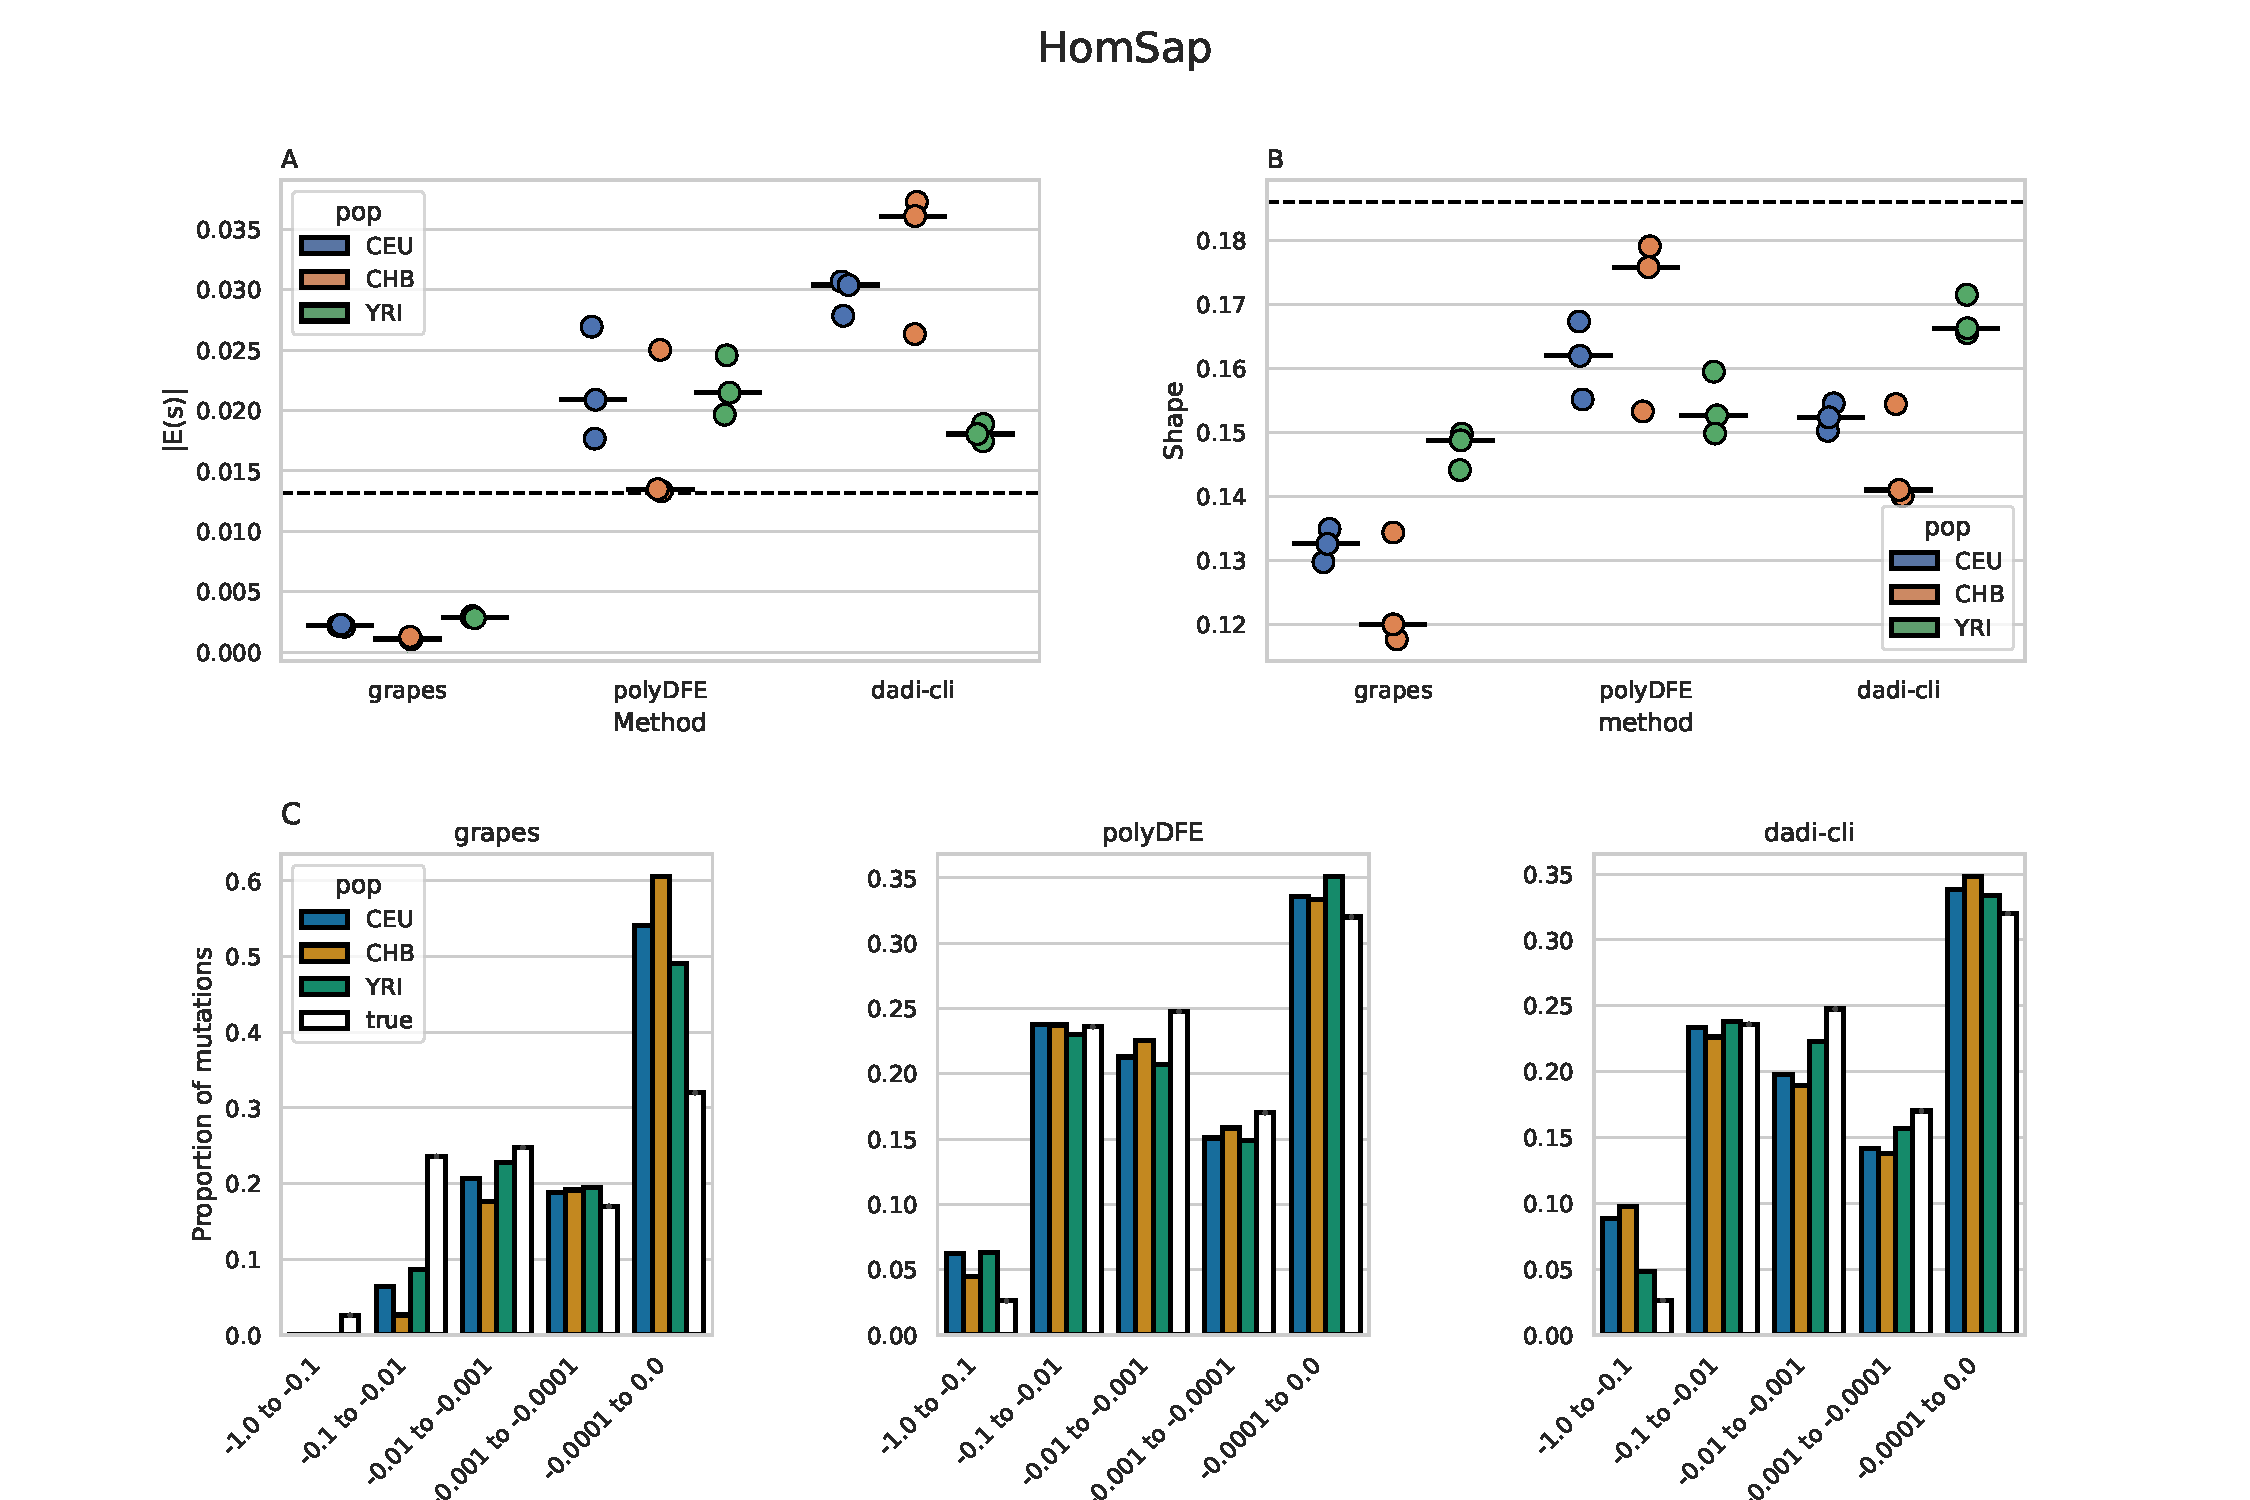
\includegraphics[width=\linewidth]{figures/HomSap/OOA/HomSap_discrete_DFE}
        \caption{Inferred versus simulated DFEs from simulated human genomes.
        Simulations were performed using a human out-of-Africa demographic model with a gamma-distributed DFE
        acting on exons (see \textbf{Methods}).
        DFE is inferred separately for each of the three extant populations (CEU, CHB, and YRI)
        by three different methods: \grapes, \polydfe , and \dadicli.
        (A-B) Mean absolute value of selection coefficient ($\lvert E(s) \rvert $) and shape parameter are
        shown for each DFE inferred from all three simulated datasets,
        with median values marked by horizontal bars
        and simulated values represented by dashed horizontal lines.
        (C) Binned distribution of $s$ implied by the average DFE inferred from the three simulated datasets (averaging the inferred gamma parameters);
        white bars represent the distribution used in the simulation.
        }
        \label{fig:homsap-dfe.ooa}
    \end{figure}



    We start by examining DFE inference from human genomes simulated under an out-of-Africa demographic model
    with selection acting on exons (see \textbf{Methods}).
    In this setting, the DFE is inferred separately for each of the three simulated populations
    using each of the three DFE-inference methods.
    In each case we note that the DFE is estimated from segregating sites only,
    without the use of substitution data, as \stdpopsim's models currently do not
    contain outgroup populations or species that can be used to estimate divergence.

    Overall, inferred DFEs varied across populations and inference methods (Figure \ref{fig:homsap-dfe.ooa}, Table \ref{tab:dfe_table}).
    Note that while the estimation accuracy for the DFE parameters themselves is informative (Figure \ref{fig:homsap-dfe.ooa}A-B),
    examining the difference between the actual and inferred distributions of $s$ can be more helpful for showing how well a method
    has recovered the true DFE (Figure \ref{fig:homsap-dfe.ooa}C).
    The distributions of $s$ inferred by \polydfe and \dadicli had higher mean values (in absolute value)
    but smaller shape parameters, while \grapes inferred distributions with lower mean values and shape parameters.
    As a result, \polydfe and \dadicli over-estimate the fraction of mutations under strong selection ($s<-0.1$),
    while \grapes considerably over-estimates the fraction of mutations under weak selection ($s\geq-0.0001$).

    Population history appears to influence different methods in slightly different ways.
    For instance, \dadicli and \grapes produce more accurate estimates from the YRI genomes
    (relative to the other two populations), whereas \polydfe
    shows very similar accuracy across all populations.
    To factor out the influence of demographic changes, we also analyzed genomes generated using similar
    simulations but with no population size changes (Figure \ref{fig:homsap-dfe.constant}, Table \ref{tab:dfe_table}).
    In this simpler setting, \polydfe overlapped the true mean selection coefficient and shape parameter, whereas
    the other methods do not show as close a correspondence.
    \grapes exhibits similar biases as observed in the simulations with more complex demography,
    but with milder under-estimation of the shape parameter,
    whereas \dadicli shows an inverse pattern
    with overestimated shape parameter and slightly underestimated mean.
    While providing possible insights into the effects of the demographic history
    on accuracy of different DFE-inference methods, substantiating these insights
    will require more than three replicate simulations per scenario.

    \begin{figure}[b!]
        \centering
        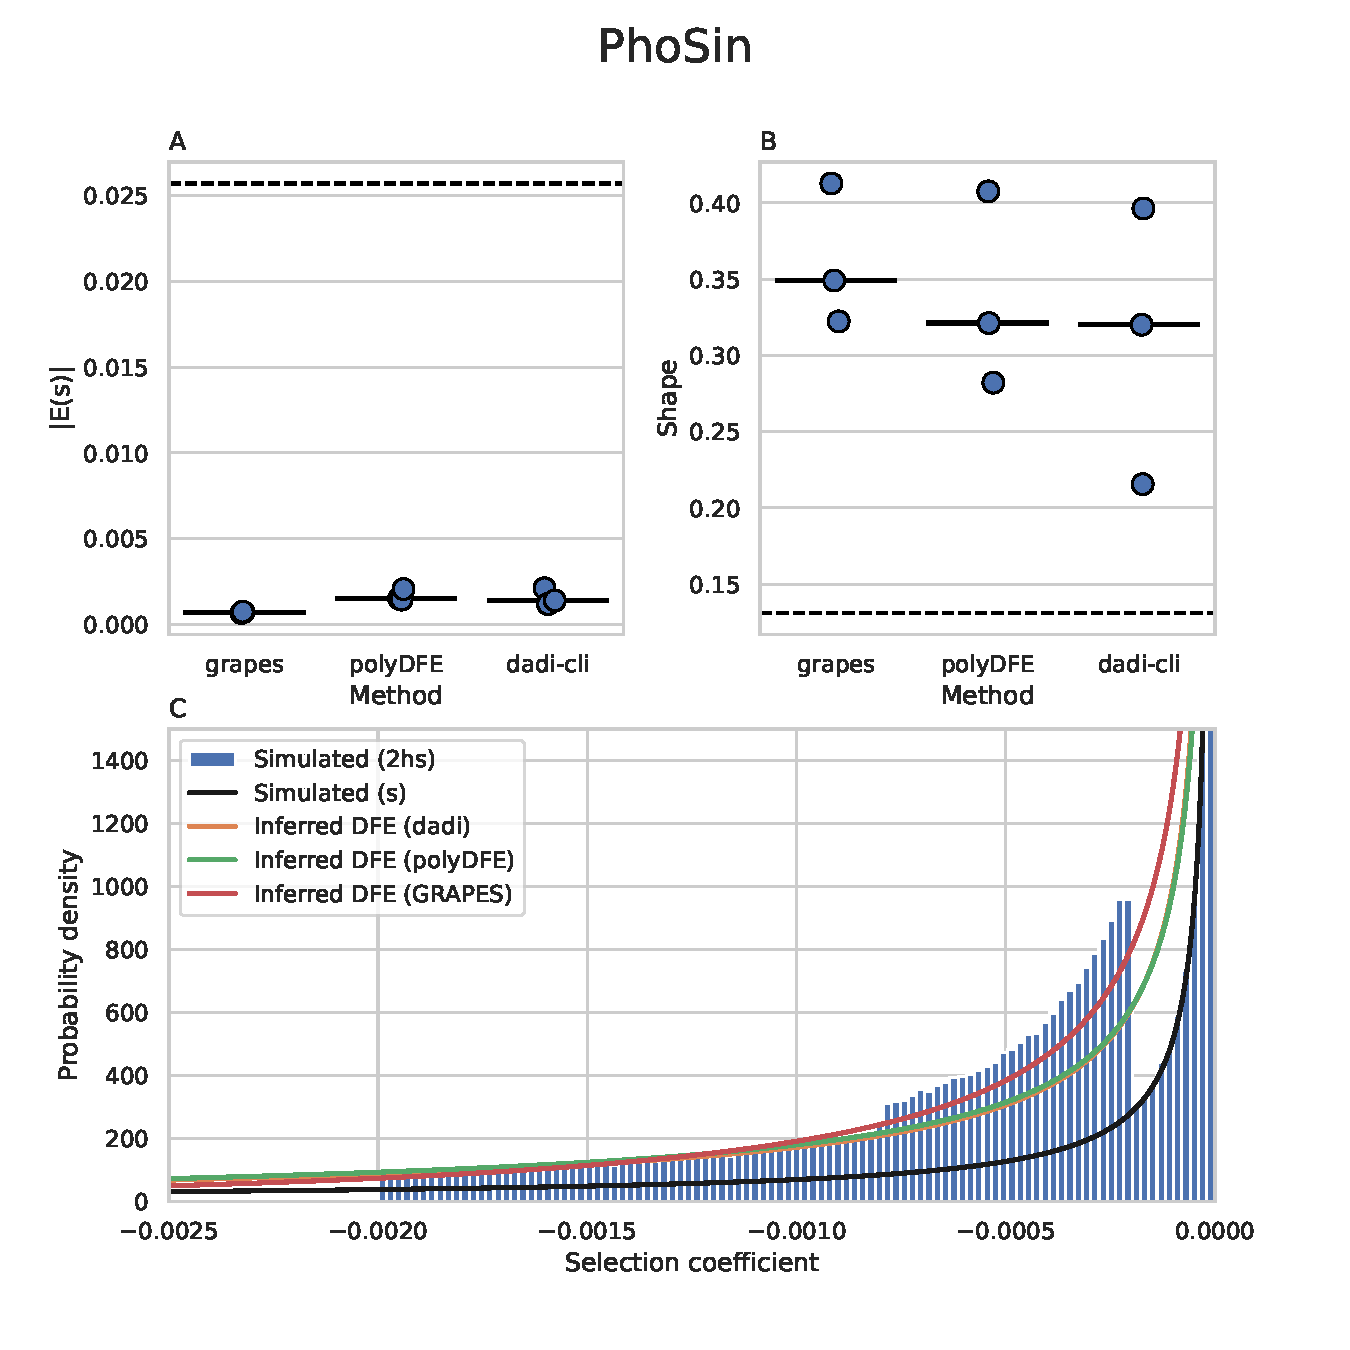
\includegraphics[width=0.8\textwidth]{figures/PhoSin/Vaquita2Epoch_1R22/PhoSin_Vaquita2Epoch_1R22_Gamma_R22_Phocoena_sinus.mPhoSin1.pri.110_exons_DFE_plot.pdf}
        \caption{
        \label{fig:vaquita-dfe}
        Inferred versus simulated DFEs from simulated vaquita genomes.
        Simulations were performed using a two-epoch model of vaquita porpoise demography with a gamma-distributed DFE
        acting on nonsynonymous mutations with a relationship between the selection coefficient ($s$) and dominance coefficient ($h$) (see \textbf{Methods}).
        The DFE is inferred by analyzing all simulated genomes jointly by one of three different methods:
        \grapes, \polydfe, and \dadicli.
        (A-B) Mean absolute value of selection coefficient ($\lvert E(s) \rvert $) and shape parameter are
        shown for each DFE inferred from all three simulated datasets,
        with median values marked by horizontal bars
        and simulated values represented by dashed horizontal lines.
        (C) Binned distribution of $2hs$ implied by the simulated DFE compared with
        the distribution of $s$ implied by the average DFE inferred for each method from the three simulated datasets (averaging the inferred gamma parameters).
        The distribution of $2 h s$ is multimodal because of the simulated relationship between $h$ and $s$ (see text).
        }
    \end{figure}

    Next, we benchmarked these three DFE-inference methods on simulations of the vaquita porpoise genome.
    Recall that these simulations apply a gamma-distributed selection coefficient to mutations in exons
    with a relationship between the selection and dominance coefficients (see \textbf{Methods}).
    In this setting, all methods perform uniformly worse than in the human genome simulations,
    with consistent underestimation of the mean selection coefficient
    and overestimation of the shape parameter (Figure \ref{fig:vaquita-dfe}A-B, Table \ref{tab:dfe_table}).
    Similar patterns are observed when re-running the simulations with a simpler demographic model
    without population size changes (Figure \ref{fig:vaquita-dfe.constant}, Table \ref{tab:dfe_table}).
    We suspect that this is due to the fact that all DFE-inference methods used here assume an additive model ($h = \frac{1}{2}$),
    while mutations in the simulated genomes were more recessive ($h < \frac{1}{2}$), and their dominance decreased with the strength of selection.
    To examine the influence of this model misspecification, we compared the inferred distributions of $s$ to the
    simulated distribution of $2hs$, which would have been equal to $s$ under an additive model (Figure \ref{fig:vaquita-dfe}C).
    Reassuringly, all three methods infer distributions that appear to fit the main mode of the simulated distribution of $2hs$.
    This is likely because deleterious alleles are typically at low frequency and thus heterozygous,
    where their selective effect is $h s$ rather than $s$.

\section*{Detection of Selective Sweeps}
    \label{sweeps}
    We next highlight how \stdpopsim can be used to benchmark and compare
    the performance of different methods for detecting selective sweeps from genetic data.
    Because simulation of selective sweeps is very time consuming and evaluation of statistical power requires
    many replicate simulations, we focused on human chromosome 1 and generated replicate simulations on 5cM segments
    %IG: took out the 7 segments with low rec rate
    of the chromosome in 93 different locations. % (see \textbf{Methods}).
    Selective sweeps were simulated by introducing a beneficial mutation in the center of the 5cM segment
    with a moderately strong selection coefficient ($s = 0.03$; $2N_es \sim 600$; see \textbf{Methods}).
    Each segment was simulated 1000 times, while keeping only replicates in which the selected allele reached a frequency of 95\% or greater.
    These sweeps were modeled in the context of the three population out-of-Africa model from \citet{gutenkunst2009inferring}
    and background selection from deleterious mutations in exons.
    Sweep-detection methods typically base their inference on checking whether a test statistic
    exceeds a certain threshold, which is determined according to some empirical null distribution.
    In our simulations, we considered two different null distributions:
    one based on neutral simulations, and another based on simulations with background selection
    from deleterious mutations in exons (see \textbf{Methods}).

     %sweeep power figure
    \begin{figure}[b!]
        \centering
        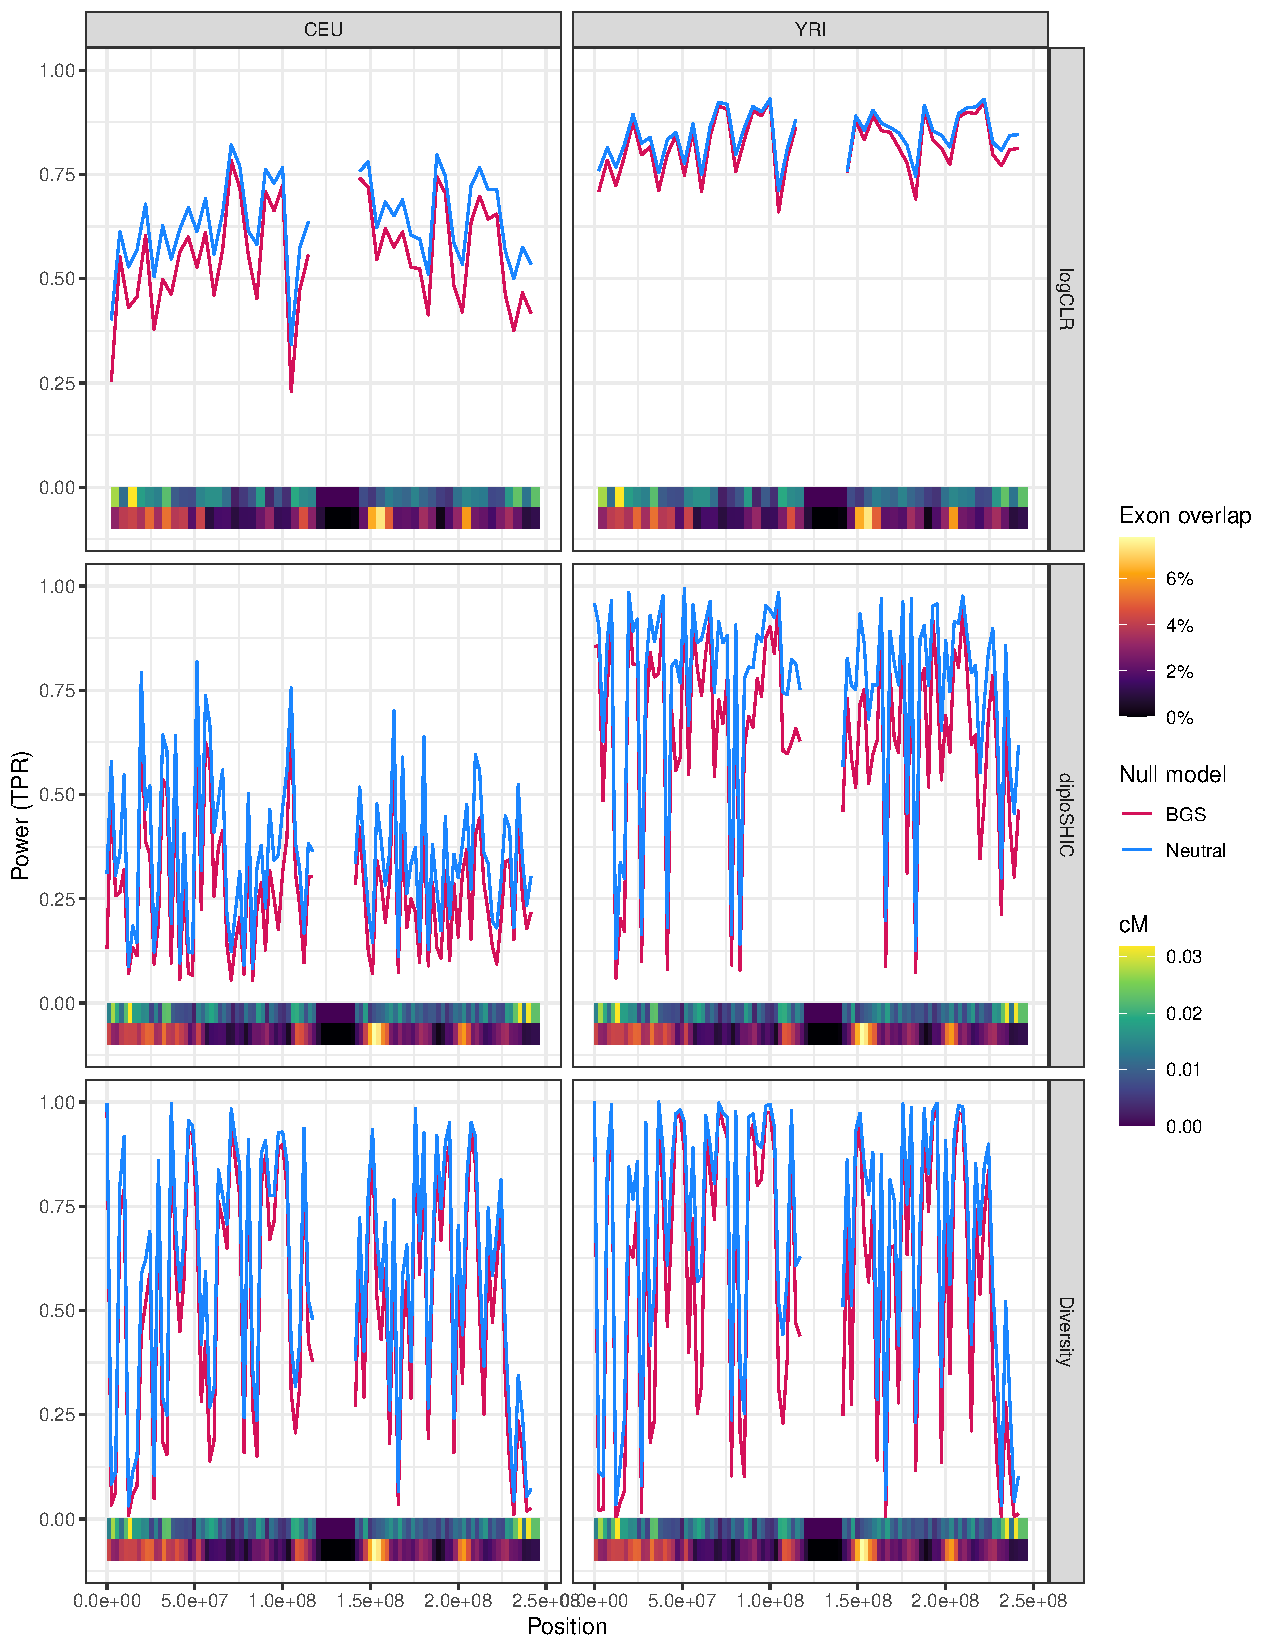
\includegraphics[width=0.8 \textwidth]{figures/sweeps/chr1_power.pdf}
        \caption{
        %IG: better not mention 100 if we're filtering out 7 segments
        %IG: removed citations from fig captions; they are prominently specified in main text
        Power to detect selective sweeps along human
        chromosome 1. Genomic segments were simulated with sweeps under a three population out-of-Africa model
        %\citep{gutenkunst2009inferring}
        and with background selection from deleterious mutations in exons.
        Three methods for detecting sweeps were applied to simulated data:
        \sweepfinder (top row -- labeled CLR),
        \diploshic (middle row),
        and reduced diversity ($\pi$) (bottom row).
        Power (true positive rate) is shown for these methods for the CEU and YRI
        samples (left and right respectively).
        The thresholds of the test statistics were set to control for
        $5\%$ false positive rate under a neutral null model (blue)
        and a null model with background selection from deleterious mutations in exons (red).
        Also shown are heatmaps of local recombination rate and exon density along the
        chromosome (bottom).
        }
        \label{fig:chr1_power}
    \end{figure}

    We evaluated the statistical power to detect selective sweeps for three methods:
    \sweepfinder \citep{degiorgio2016sweepfinder2},
    \diploshic \citep{kern2018diplos},
    and reduced diversity ($\pi$).
    For each method, we determined a threshold for its test statistic
    using each of the two null models separately -- neutral and with background selection (BGS)
    -- and controlling for a $5\%$ false positive rate.
    %
    We then applied each method to data simulated with sweeps for two samples (YRI and CEU)
    in each of the simulated locations along human chromosome 1 (Figure \ref{fig:chr1_power}).
    First and most strikingly, the power to detect sweeps varies considerably along the chromosome,
    and this variation is much greater than the variation in power between CEU and YRI or between
    null models. This is likely due to the effects of recombination rate heterogeneity (Figure \ref{fig:chr1_power}).
    Next, we notice that power to detect sweeps is slightly lower when the test statistic threshold
    is determined using simulated data with background selection (BGS null model).
    This is likely because the strength of selection acting on exons is relatively weak, and the
    sweep detection methods we have used are relatively robust to the effects of background selection.
    Finally, the power to detect sweeps is generally higher in the YRI sample
    than in the CEU sample, which is consistent with the fact that YRI has a larger ancestral effective population size and
    thus both stronger selection and more variation to detect a sweep \citep[e.g.,][]{simonsen1995properties}.
    Conversely, the CEU population experienced the out-of-Africa bottleneck that may mute the signal of a sweep.

    We compared the overall performance of the three sweep-detection methods using
    receiver operating characteristic (ROC) curves (Figure \ref{fig:roc-curves}).
    Performance varies for each of the sampled populations.
    In the CEU sample, \sweepfinder and \diploshic perform similarly with a high area under the curve (AUC) score,
    (AUC = 0.906 and 0.903 respectively), but both underperform the simple method
    that uses reduced diversity ($\pi$) as an indicator (AUC = 0.932).
    In the YRI sample, \diploshic outperforms the other two methods,
    with an AUC of 0.979, followed by using outliers of $\pi$ with an AUC of 0.957,
    and then \sweepfinder with an AUC of 0.939.
    We note that we trained \diploshic on simulations under a constant size population,
    which more closely matches the demographic history of YRI, than that of CEU, which
    is characterized by a strong recent bottleneck followed by population expansion.
    Interestingly, the simple method that uses reduced diversity ($\pi$) as an indicator
    for a selective sweep performs very well overall (especially on the CEU sample).
    However, its accuracy is much more variable along the chromosome compared to the other two methods (see Figure \ref{fig:chr1_power}),
    and for quite a few locations along the chromosome it has power below $50\%$
    when applied to both sample sets.
    \sweepfinder appears to have the least variation in power along the chromosome or across populations.




    \begin{figure}[b!]
        \centering
        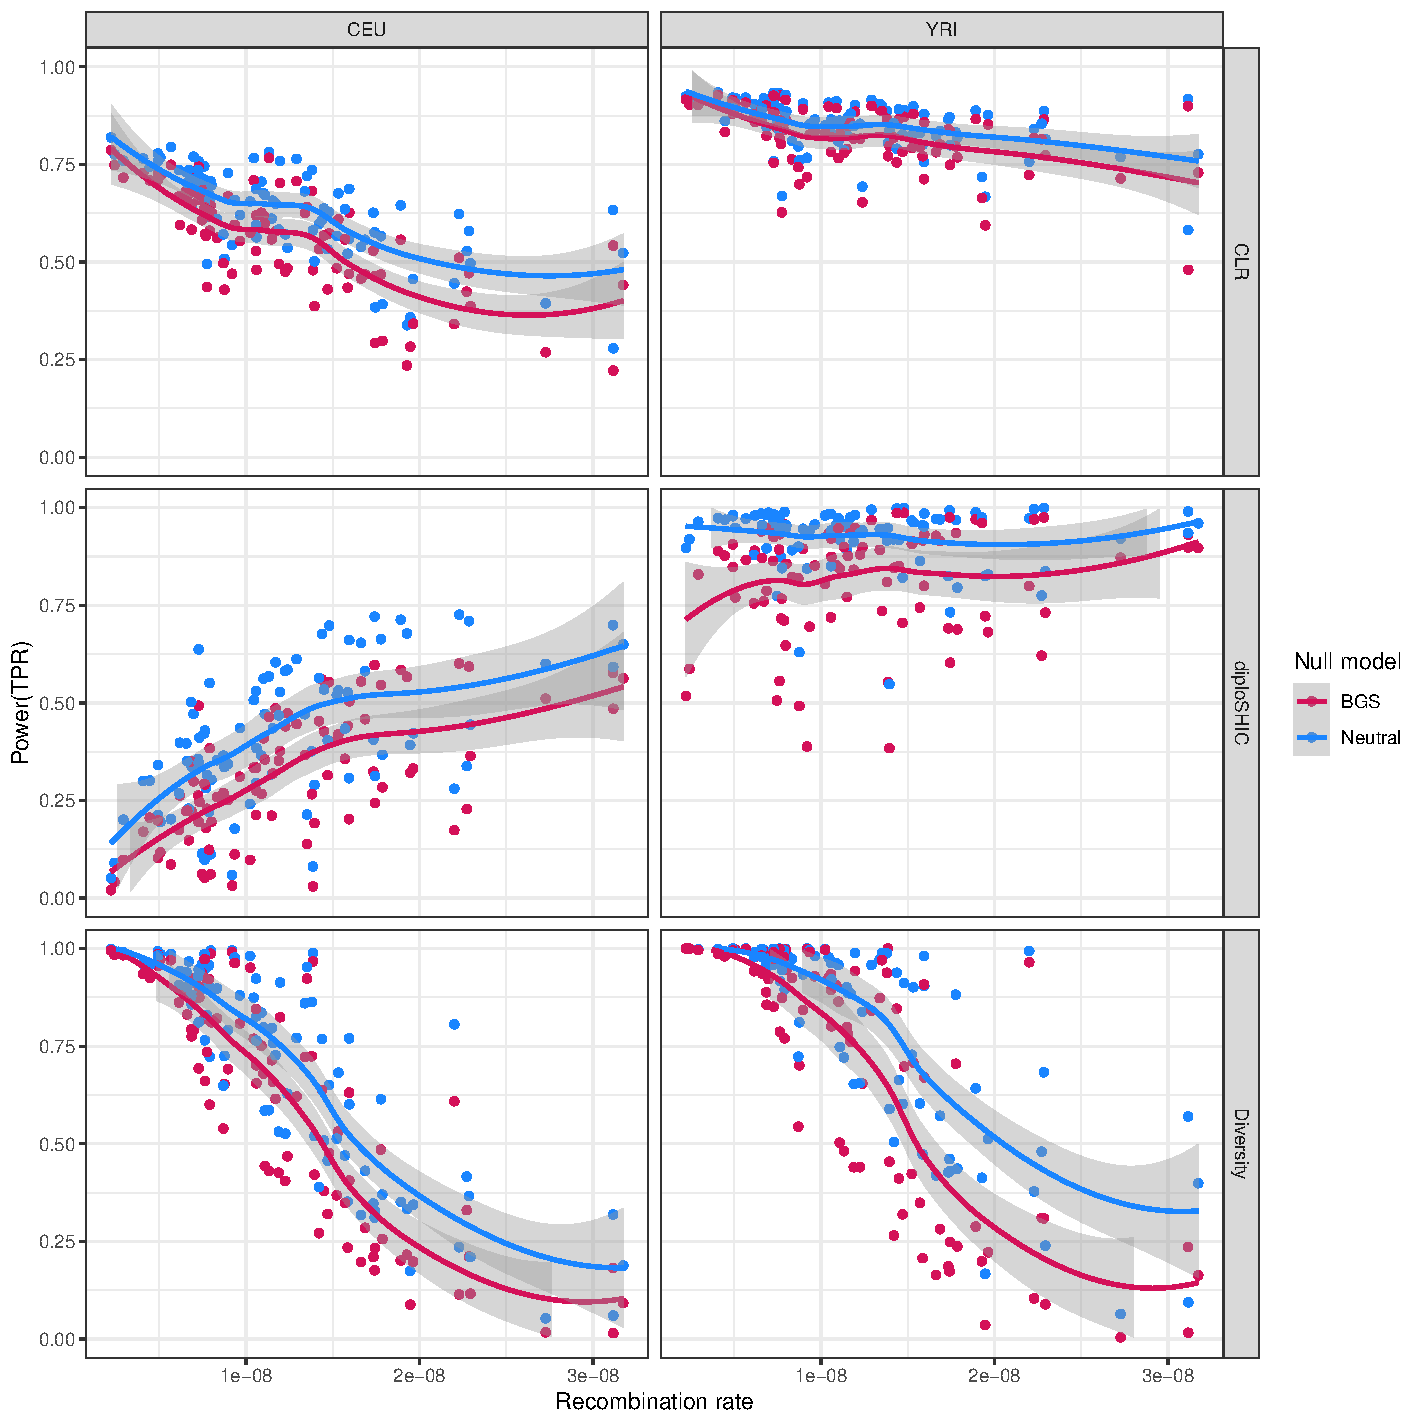
\includegraphics[width=0.8 \textwidth]{figures/sweeps/relationship_power_cM.pdf}
        \caption{
        Power to detect selective sweeps
        as a function of local recombination rate.
        This figure shows the same power estimates shown in Figure \ref{fig:chr1_power},
        but with the genomic segments plotted against their
        average recombination rates instead of position along chromosome 1.
    	Genomic segments were simulated with sweeps under a three population out-of-Africa model
        and with background selection from deleterious mutations in exons.
        Three methods for detecting sweeps were applied to simulated data:
        \sweepfinder (top row-- labeled CLR),
        \diploshic (middle row),
        and reduced diversity ($\pi$) (bottom row).
        Power (true positive rate) is shown for these methods for the CEU and YRI
        samples (left and right respectively).
        The thresholds of the test statistics were set to obtain a
        $5\%$ false positive rate under a neutral null model (blue)
        and a null model with background selection from deleterious mutations in exons (red).
        Fitted lines represent loess smoothed regressions.
        }
        \label{fig:power-recomb}
    \end{figure}

    To further dissect the reasons for high variance along the chromosome in power to detect sweeps,
    we examined the relationship between power and local recombination rate (Figure \ref{fig:power-recomb}).
    We see that power to detect sweeps is
    a decreasing function of local recombination rate for \sweepfinder and reduced diversity,
    which is consistent with sweeps having a larger genomic footprint in regions of low
    recombination.
    \diploshic on the other hand shows a slight increase in power with recombination rates,
    presumably because it is designed to distinguish regions where a sweep happened from regions linked to a sweep,
    and if the recombination rate is too low (or selection too strong) then the genomic window examined by \diploshic may
    not be large enough to exhibit enough of a recovery in patterns of diversity flanking the sweep.
    These results confirm that reduced genetic diversity performs well as an indicator for selective sweeps only in regions with
    low recombination rate.
    The other two methods, which were specifically designed for sweep detection, are considerably more robust
    to the effects of recombination rate than the simple indicator of reduced genetic diversity.
    These methods are particularly robust to recombination rate variation when applied to
    the YRI sample, especially when using a neutral null model to calibrate the test statistics.
    The other null model, which assumes background selection from exons,
    appears to consistently lead to reduced power for detecting sweeps regardless of the recombination rate.
    Interestingly, we do not see a clear correlation between power to detect sweeps and
    local exon density (Figure \ref{fig:power-exon}).
    This is somewhat surprising given that background selection is expected to somewhat interfere with the sweep signature.
    This might suggest that the effects of realistic background selection on genome variation
    may not be as similar to those of sweeps as previously thought \citep{schrider2020background}.

\section*{Discussion}
    \label{Discussion}
    In this paper, we have presented an important new addition to the \stdpopsim{} library
    that allows for simulating genetic variation in the presence of selection.
    We have demonstrated the utility of this new API by showing how it can be used to benchmark
    the performance of different methods for demographic history inference, the inference of the distribution
    of fitness effects of new mutations, and the detection of selective sweeps.
    This allows for a wide range of models of selection to be easily simulated and compared to
    empirical data, with reproducibility, computational efficiency, and rigor.

    The exploration of performance among methods done here is not meant to be thorough
    benchmarking, but rather to highlight the utility of the \stdpopsim resource.
    Having said that, there are a number of interesting results that bear discussion.
    The first pertains to estimation of demographic history ($N_e(t)$) in the context of
    linked purifying selection. Our simulations of humans and vaquita genomes
    model deleterious mutations only at exonic positions of the genome.
    As shown in Figures \ref{fig:homsap-summary-stats} and \ref{fig:vaquita-summary-stats},
    this combination only produces sizable decreases in polymorphism at exonic positions,
    which represent a small minority of sites within the genome, and does not lead to large-scale
    perturbations in genome-wide diversity. Thus, it is not surprising that estimates of $N_e(t)$
    from genome-wide data from which exons have been masked should be accurate
    (e.g., Figures \ref{fig:human-demography} and \ref{fig:vaquita-demography}).
    However, the question remains to what extent this would be true in empirical data where
    selection is not constrained to coding positions. For instance, we know
    that many genomes harbor large numbers
    of conserved non-coding elements \citep[e.g.,][]{siepel2005evolutionarily} with extremely
    strong selection acting on them \citep{katzman2007human,mclean2008dispensability}.
    We thus caution extrapolating from our results. Future studies might build upon
    the annotations we used here to include selection at other portions of the genome as well
    as mixtures of DFEs across sites.

    A second important finding is that inference of the DFE
    is sensitive to the dominance of deleterious mutations.
    All three of the DFE-inference methods applied here assume that deleterious mutations act
    in an additive fashion ($h=0.5$) by default.
    However, the simulated DFE for the vaquita genome included highly recessive mutations.
    Specifically, these simulations used a DFE where mutations with $s<-0.01$ are quite recessive,
    with $h<=0.01$, and where mutations with $-0.01<s<-0.001$ have $h=0.1$.
    We found that the three DFE-inference methods underestimated $E[s]$ and overestimated the shape parameter (Figure \ref{fig:vaquita-dfe}A-B).
    This performance is not surprising as decreasing $h$ for a given distribution of $s$ will lead to a decrease in $hs$,
    or an apparent decrease in the amount of selection.
    Fitting a mis-specified DFE that assumes $h=0.5$ will then lead to underestimates of $E[s]$.
    Indeed, the distribution of $hs$ is much more accurately estimated (Figure \ref{fig:vaquita-dfe}C).
    Overall, these results are consistent with prior work showing that it is challenging to separately
    infer the DFE of $s$ along with $h$ \citep{veeramah2014evidence, kyriazis2024constraining, balick2022overcoming}
    and that a large proportion ($>5\%$) of recessive deleterious mutations can confound inferences of $s$ \citep{wade2023quantifying}.
    Given the plethora of evidence for recessive deleterious mutations
    \citep{mukai1972mutation, agrawal2011inferences, huber2018gene, di2024revisiting},
    these results suggest the need for care in DFE inference.
    Kyriazis and Lohmueller \citeyear{kyriazis2024constraining} inferred the DFE of $s$ for nonsynonymous mutations
    in humans when considering different values of $h$.
    Intriguingly, additive models showed a satisfactory fit to the SFS of nonsynonymous variants in humans
    and more complex models of dominance did not substantially improve the fit.
    Nevertheless, models including recessive deleterious mutations, like those simulated here for the vaquita genome,
    show a similar fit to the SFS and may be more biologically realistic than fully additive models,
    given the evidence for the presence of recessive deleterious mutations.
    More broadly, new computational approaches are needed to precisely quantify the DFE and the covariance of $h$ and $s$.

    Further, inference of the DFE was done here using exon annotations of the genome in question.
    A key distinction between our analyses and those done in practice
    is that we have complete knowledge of which sites are under selection in the simulation,
    thus our inferences represent a best case scenario. Empirical inference of the DFE is a much
    harder problem as some mutations assumed to be free of selection
    may in reality be under selection and strength of selection can change over time or with environment.

    Regarding sweep detection, the inclusion of selection models into \stdpopsim allowed us to readily compare the
    effectiveness of different methods on data reflecting the demographic history, recombination rate variation,
    and genomic locations of negatively selected sites present in human populations. These results clearly demonstrate
    the impact of recombination rate variation, and underscore the importance of training methods on data with variable
    recombination rates \citep[e.g.,][]{schrider2017soft}. In addition, our results
    illustrate a strength of likelihood methods like \sweepfinder, that do not require a predefined window size.
    Window-based methods, such as \diploshic, tend to lag in performance when the genomic region affected by the sweep is
    larger than the chosen window size, as can occur with very strong sweeps or low levels of
    recombination. Moreover, while all the methods examined here retain adequate power for sweep identification across
    scenarios, including the inclusion of background selection, our results underscore the importance of developing
    methods that are well powered in the face of unknown demographic histories. Indeed, larger differences
    in power were observed when applying a method to genomes simulated with different demographic histories (i.e., YRI versus CEU)
    than when calibrating a method using a null model with and without background selection.

    Although we have shown how the new \stdpopsim API can be used to benchmark the performance of different methods,
    the benchmarks shown here merely scratch the surface of what can be done with the new API.
    We envision that, moving forward, many researchers will use
    the new API to simulate data under a wide range of models of selection, demography, and genome architecture, and to develop
    new methods for the analysis of genetic data in the presence of selection.
    The additions described here further expand the utility of \stdpopsim for both
    characterizing the patterns of diversity expected under a wide range of population genetic
    models, and for benchmarking methods for the analysis of genetic data
    on common ground in a way that was not possible before.

\section*{Methods}
    \label{methods}

    \subsection*{Annotations}
    Currently available annotation data in \stdpopsim were downloaded from Ensembl.
    Coding sequence and exon annotations are available for
    \textit{Arabidopsis thaliana} \citep{cheng2017araport},
    \textit{Drosophila melanogaster} \citep{hoskins2015release},
    \textit{Homo sapiens} \citep{hunt2018ensembl},
    and \textit{Phocoena sinus} \citep[vaquita porpoise,][]{morin2021}.

    \subsection*{Quality control and software development}
    Following the protocol established previously for other aspects of \stdpopsim{} \citep{adrion2020community},
    new DFEs are subject to a rigorous quality control (QC) process,
    by which a separate individual re-implements the same DFE, and the two implementations
    are programmatically tested for equality.
    %IG: tried to put a more positive spin on the DFE bug example
    This QC process has proven its effectiveness in numerous occasions in detecting implementation bugs
    and resolving modeling ambiguities.
    For example, this process detected  an error in coding the log-normal distribution of
    the \textit{Drosophila melanogaster} DFE inferred by \citet[\stdpopsim label \texttt{LognormalPlusPositive\_R16}]{booker2021selective}.
    This faulty DFE model was used in a study conducted by one of our groups before it underwent the QC process,
    where we noticed that deleterious selection coefficients
    were several orders of magnitude larger than expected.
    Subsequently, the QC process was able to find and fix this bug.
    In addition to QC, all changes and additions to the code must pass a comprehensive set of unit tests:
    at the time of writing, the library includes over 11,000 lines of testing code,
    that run 2,862 unit tests, including comparisons to QC implementations
    and cross-checks for agreement, including between \slim and \msprime implementations of the same models.
    For instance, for testing we make use of \slim's scriptability to separately record as metadata
    the simulation parameters (current population sizes, DFEs, etc.),
    which are then programmatically compared to the models used to generate the \slim script
    that ran the simulation.
    We make use of automatic test ``code coverage'' tools to help ensure that all portions of the code base
    are validated by these unit tests.

    \subsection*{Whole genome simulations}
    In this study we performed simulations of the human and vaquita porpoise genomes
    using \stdpopsim{}. We ran replicate simulations for each genome/parameter combination,
    in which chromosomes were simulated separately from one another.
    All simulations were executed using the \slim engine with a burn-in of $10N$ generations
    (where $N$ is the initial population size), and a scaling factor of 1 (no scaling).
    All simulations were implemented using a \snakemake workflow,
    where the code utilized is similar to that shown in Figure~\ref{fig:schematic}B.
    The complete simulation workflow is available at \url{https://github.com/popsim-consortium/analysis2/blob/main/workflows/simulation.snake}
    (see \textbf{Data availability} below).


    \subsubsection*{Simulations of complete human genomes}
    Simulation of human genomes used a genetic map from the HapMap Project
    \citep[\stdpopsim label \texttt{HapMapII\_GRCh38}]{international2007second} and
    the out of Africa demographic model with archaic admixture from
    \citet[\stdpopsim label \texttt{OutOfAfricaArchaicAdmixture\_5R19}]{ragsdale2019models}.
    Simulations with selection additionally applied a DFE model with gamma-distributed selection coefficients inferred by
    \citet[\stdpopsim label \texttt{Gamma\_K17}]{kim2017inference} to exons annotated by the HAVANA group release 104
    \citep[\stdpopsim label \texttt{ensembl\_havana\_104\_exons}]{ensembl2018}.
    Each simulation generated 100 diploid genomes from each of three extant human populations (labeled YRI, CEU, and CHB),
    with each genome consisting of 22 autosomes.
    Using these settings, we generated three replicate datasets without selection
    and three replicate datasets with selection.
    Three additional datasets, used in Figure \ref{fig:homsap-dfe.constant},
    were simulated with the same model of selection and a simple demographic model with one population with a constant size of $10,000$.
    Each of these simulations generated 100 diploid genomes.
    The configuration file used in combination with our \snakemake workflow
    for these simulations can be found at \url{https://github.com/popsim-consortium/analysis2/blob/main/workflows/config/snakemake/production_config_HomSap.yml}.

    \subsubsection*{Simulations of complete vaquita porpoise genomes}
    Simulation of vaquita porpoise genomes used
    the two-epoch demographic model from \citet[\stdpopsim label \texttt{Vaquita2Epoch\_1R22}]{robinson2022critically}.
    Since no genetic map is currently available for this species, we assumed a constant recombination rate of $10^{-8}$
    across all chromosomes \citep{morin2021}.
    Simulations with selection additionally applied a DFE model with gamma-distributed selection coefficients inferred by
    \citet[\stdpopsim label \texttt{Gamma\_R22}]{robinson2022critically} to exons annotated from the vaquita porpoise genome assembly
    \citet[\stdpopsim label \texttt{Phocoena\_sinus.mPhoSin1.pri.110\_exons}]{morin2021}.
    This DFE model implements a relationship between selection and dominance as follows:
    very deleterious mutations (with $s<-0.1$) are recessive ($h=0$),
    mutations with $s\in [-0.1,-0.01)$ have a dominance coefficient of $h=0.01$,
    mutations with $s\in [-0.01,-0.001)$ have a dominance coefficient of $h=0.1$,
    and very mild mutations (with $s\in [-0.001,0)$) are nearly additive ($h=0.4$).
    This discretized relationship matches that used by \textcite{robinson2022critically},
    and is easily implemented in \stdpopsim's \texttt{DFE} class.
    Each simulation generates 100 diploid genomes,
    with each genome consisting of 21 autosomes.
    Using these settings, we generated three replicate datasets without selection
    and three replicate datasets with selection.
    Three additional datasets, used in Figure \ref{fig:vaquita-dfe.constant},
    were simulated with the same model of selection and a simple demographic model with one population with a constant size of $3,500$.
    The configuration file used in combination with our \snakemake workflow
    for these simulations can be found at
    \url{https://github.com/popsim-consortium/analysis2/blob/main/workflows/config/snakemake/production_config_PhoSin.yml}.


    \subsection*{Inference of $N_e(t)$}
    Inference of $N_e(t)$ was conducted on simulated datasets after masking non-recombining portions
    of the genome (to avoid bias caused by extreme recombination rate variation)
    and exons (to avoid the direct effect of natural selection).
    Thus, inference from datasets simulated with selection was not influenced by direct selection
    acting on exons, but it was influenced by selection acting on linked sites (background selection).
    %
    We assessed the accuracy of demographic inferences from four software packages:
    \msmc \citep{Schiffels2020}, \stairway \citep{liu2020stairway}, \gone \citep{santiago2020recent},
    and \smcpp \citep{terhorst2017robust}.
    For \msmc
    we used a random sample of $N=6$ simulated genomes with 20
    iterations of the EM algorithm.
    For \gone we set \texttt{max\_snps} to 500,000,
    the number of generations to 2,000, and the number of bins to 400, all representing default settings.
    For \stairway we did one run of $\theta$ estimation for each replicate dataset,
    and used a \texttt{dimFactor} of 5000, both of which represent default settings.
    For \smcpp we used the unfolded SFS (\texttt{--unfold}),
    along with the true mutation rate under which the simulations were generated.
    The complete \snakemake workflow for demographic inference can be found at
    \url{https://github.com/popsim-consortium/analysis2/blob/main/workflows/n_t.snake}.


    \subsection*{DFE inference}
    % ADK: I've tried to deal with all the comments here
    We used three software packages to infer the distribution of fitness effects (DFE) from genetic data:
    \dadicli \citep{Huang2023,kim2017inference}, \polydfe \citep{tataru2020polydfe}, and \grapes \citep{galtier2016adaptive}.
    Each software package was run using the same set of simulations.
    DFE inference using \dadicli was conducted by first inferring a demographic model from neutral sites,
    using a two epoch demographic model with 100 repeated runs of the optimization procedure.
    \dadicli then proceeds by using a cached strategy wherein we used 2000 points in the gamma distribution.
    Finally, the DFE was inferred using a ratio of non-synonymous to synonymous mutations of 2.31, again with
    100 repeated runs of the optimization procedure.
    For \polydfe, we used model `C' which uses a mixture of a gamma distribution and an exponential distribution,
    where the gamma component is used for negatively selected mutations. For optimization we used
    the default BFGS optimizer with the \texttt{-e} flag to automatically estimate the initial parameters values.
    For \grapes, we inferred the DFE under the `GammaZero' model, which assumes that selection coefficients
    are drawn from a single gamma distribution. We used the \texttt{-no-div-param} flag to disable the use
    of divergence-based parameter estimation. All other settings were left at their default values.
    All methods used the same exon annotations as generated in the simulations. The total number of coding sites
    in the human and vaquita genomes used were 61,644,801 and 31,039,513 respectively.

    % ADK: I've added a section below that describes the DFE inference methods used in this study.
    To facilitate direct comparison between inference methods,
    we scale each program's output to obtain a selection coefficient ($s$) consistent with the one used by \slim.
    %IG: expanded a bit to justify each scaling decision
    \grapes outputs the mean and shape of the inferred distribution of $4N_es$.
    We thus scale the mean by a factor of  $\frac{\mu}{\theta}$,
    where $\mu$ is the assumed mutation rate and
    $\theta=4N_{e}\mu$ is the population-scaled mutation rate, as estimated by \grapes.
    \polydfe is similarly scaled by $\frac{2\mu}{\theta}$,
    reflecting the fact that it defines the selection coefficient such that a homozygote has fitness $1+ 2s$.
    \dadicli infers a gamma distribution for $N_es$ and parameterizes this distribution using the shape ($\alpha$) and rate ($\nu$).
    %IG: we're still missing justification for the scaling by L and p, but we can leave this for revision
    Thus, the mean value of $s$ is obtained by  $\frac{4\mu}{\theta} \alpha \nu L p$,
    where $L$ is the total number of sites available for the analysis,
    and $p$ is the proportion of sites under selection.
    Complete details for the DFE inference analysis can be found in the
    \snakemake workflow at \url{https://github.com/popsim-consortium/analysis2/blob/main/workflows/dfe.snake}.



    \subsection*{Simulations with selective sweeps}

    To test methods for detecting selective sweeps, we considered 100 evenly distributed 5cM
    segments of human chromosome 1.
    As recombination rate varies across the genome, the size of the region in base pairs simulated varied, however the recombination distance,
    which is critical for the linked effects of a sweep, was held constant.
    %IG: moved this up here since it makes mroe sense to describe it as if these segments were never simulated
    % also converted to rec rate from cM. Please check!
    Seven segments in which the central 1Mb had an average recombination rate below $10^{-11}$ were excluded from the analysis.
    Each segment was simulated in each of the following three settings:
    (1) neutral, (2) background selection (BGS), and (3) hard sweep with BGS.
    In all three settings, we applied a genetic map from the HapMap Project
    \citep[\stdpopsim label \texttt{HapMapII\_GRCh38}]{international2007second} and
    the three-population out of Africa (OOA) demographic model from
    \citet[\stdpopsim label \texttt{OutOfAfrica\_3G09}]{gutenkunst2009inferring}.
    In the two settings with BGS, we applied the DFE model with gamma-distributed selection coefficients inferred by
    \citet[\stdpopsim label \texttt{Gamma\_K17}]{kim2017inference} to exons annotated by the HAVANA group release 104
    \citep[\stdpopsim label \texttt{ensembl\_havana\_104\_exons}]{ensembl2018}.
    Hard sweeps were modeled by generating a single beneficial mutation
    with selection coefficient of $s = 0.03$ in the center of the 5cM genomic segment
    and discarding simulations in which the beneficial mutation did not reach (or exceed) a terminal frequency of $95\%$.
    For each of the 93 genomic segments of chromosome 1, we generated 1,000 replicate datasets under each of the three settings.
    We used the \slim engine with a burn-in of $2N$ generations
    (where $N$ is the initial population size), and a scaling factor of 2.
    Each simulation generated ten diploid genomic segments for each of the two sampled populations: YRI and CEU.
    The sequences simulated with a hard sweep and BGS were used for sweep detection,
    and sequences simulated under the other two settings were used to calibrate the thresholds of the test statistics
    used by the three sweep-detection methods (see below).

    \subsection*{Selective sweeps detection}

    Each of the three sweep-detection methods is based on a test statistic.
    Reduced nucleotide diversity is based on nucleotide diversity  ($\pi$)
    computed directly from the underlying tree sequences using \tskit \citep{ralph2020efficiently}
    over ten equally sized and non-overlapping subwindows.
    \sweepfinder \citep{degiorgio2016sweepfinder2} is based on a composite likelihood ratio (CLR)
    computed at 21 uniformly distributed positions along the simulated region.
    \diploshic \citep{kern2018diplos} uses supervised learning to train a sweep classifier.
    Its training phase used \texttt{discoal} \citep{kern2016discoal} to simulate 20 haploid sequences of length 1.21Mbp
    with a constant population size of $N_e=10,000$, a mutation rate of $2\times 10^{-8}$, and a recombination rate of $2\times 10^{-8}$.
    For \texttt{discoal} simulations that included selective sweeps,
    selection coefficients were drawn from a uniform distribution between $0.001$ and $0.10$,
    and the time of the sweep was chosen from a uniform distribution between $0$ and $0.01N_e$ generations in the past.
    For soft sweeps, the frequency at which selection was introduced was drawn from a uniform distribution between $0.0001$ and $0.1$.
    We note that since the training set of \diploshic was generated under a simple model with
    constant mutation and recombination rates and constant effective population size,
    we expect it to perform suboptimally on the simulated segments of human chromosome 1,
    which were generated using more realistic simulations (see \textbf{Simulations with selective sweeps} above).

    The three sweep-detection methods were associated with thresholds for their respective test statistics
    ($\pi$, \sweepfinder's CLR, or \diploshic's probability),
    which were determined using an empirical distribution representing a null model without sweeps.
    We considered two null models: a neutral evolution model (neutral),
    and a model with background selection from deleterious mutations in exons (BGS).
    %IG: deducted 7000 datasets for the low-rec regions
    Each null model was represented by a different set of $93,000$ simulations generated according to the appropriate model
    (see \textbf{Simulations with selective sweeps} above).
    Thus, for each test statistic we determined two thresholds corresponding to these two different null models (neutral and BGS)
    using the extreme $5\%$ quantile in each empirical distribution.
    Then, power (or true positive rate) to detect a sweep by a given method was determined for
    positions on chromosome 1 as follows:
    %IG: the 1000 simulations are with hard sweep + BGS
    each sweep-detection method was applied to the 1,000
    simulated datasets generated with a hard sweep and BGS for that position,
    and the power was set to be the proportion of simulations (out of 1,000)
    in which the test statistic exceeded the threshold determined by each of the two null models (neutral and BGS).
    We note that using an empirical distribution to determine the threshold for calling a selective
    sweep with \diploshic deviates from the original implementation of the method,
    however for consistency among methods we chose to take this approach.
    The complete \snakemake workflow for sweep detection (including simulations) can be found at
    \url{https://github.com/popsim-consortium/analysis2/blob/main/workflows/sweep_simulate.snake}.

\section*{Data availability}\label{data_availability}
The release of \stdpopsim is available at \url{https://github.com/popsim-consortium/stdpopsim}.
This paper coincides with version 0.3.0 of \stdpopsim.
The entire analysis pipeline associated with this paper is available
as a \snakemake workflow at \url{https://github.com/popsim-consortium/analysis2}.

\section*{Acknowledgments}\label{acknowledgements}
We thank Tom Booker for discussions and encouragement to incorporate realistic BGS models into \stdpopsim.
We thank the numerous users of the \stdpopsim package and well as
workshop participants who provided feedback and suggestions for improvements.

\section*{Funding}
    \label{funding}
    % we got too many people to do initials
    M.~Rodgrigues, S.~Tittes, N.~Pope, and A.~Kern were supported in part by NIH award R35GM148253.
    R.~Gutenkunst and L.~Tran were supported in part by NIH award R35GM149235.
    D.~Schrider was supported in part by NIH award R35GM138286.
    K.~Lohmueller was supported by NIH award R35GM119856.
    P.~Ralph, B.~Haller, J.~Kelleher, and A.~Kern
    were supported in part by NIH award R01HG012473.
    G.~Gorjanc and Y.~Zhang were supported in part by BBSRC (BBS/E/RL/230001A, BBS/E/RL/230001C, BB/T014067/1),
    Chinese Scolarship Council (CSC) and Genus.
    C ~Huber was supported by NIH award R35GM146886.

\printbibliography

%%%%%%%% supplementary material
\clearpage
\beginsupplement

\section*{Supplementary Material}

%IG: moved supp table here, because otherwise it appeared between the supp figs
%IG: edited caption and removed annotations column, since they're all exons now.
%IG: moved commented "all sites" rows to bottom
\begin{table}[h]
\centering
\small

\caption{\textbf{Performance of DFE-inference methods in four simulation scenarios}.
For each of the three methods, we report the mean absolute error (MAE) of the mean selection coefficient and shape of its inferred DFE.
In each simulation scenario, the lowest MAEs are highlighted in bold.}

\begin{tabular}{lllrrrrrr}
\toprule
species ID & demography & \makecell{MAE \\ $E|s|$ \\ dadi-cli} & \makecell{MAE \\ $E|s|$ \\ grapes} & \makecell{MAE \\ $E|s|$ \\ polyDFE} & \makecell{MAE \\ shape \\ dadi-cli} & \makecell{MAE \\ shape \\ grapes} & \makecell{MAE \\ shape \\ polyDFE} \\
\midrule
HomSap & Constant  & \bf{0.0012} & 0.0101 & 0.0023 & 0.030 & 0.0086 & \bf{0.0068} \\
HomSap & OOA 5R19  & 0.014 & 0.0111 & \bf{0.0072} & 0.031 & 0.051 & \bf{0.024} \\
PhoSin & Constant  & 0.024 & 0.025 & 0.024 & \bf{0.23} & 0.25 & 0.23 \\
PhoSin & Vaquita2Epoch 1R22  & 0.024 & 0.025 & \bf{0.024} & \bf{0.18} & 0.23 & 0.21 \\
%HomSap & Constant & all sites & 0.0027 & 0.0111 & \bf{0.0018} & \bf{0.00071} & 0.029 & 0.014 \\
%HomSap & OOA 5R19 & all sites & 0.012 & 0.012 & \bf{0.0074} & \bf{0.027} & 0.055 & 0.035 \\
%PhoSin & Constant & all sites & \bf{0.024} & 0.025 & 0.024 & 0.21 & 0.24 & \bf{0.19} \\
%PhoSin & Vaquita2Epoch 1R22 & all sites & \bf{0.024} & 0.025 & 0.024 & 0.20 & 0.23 & \bf{0.18} \\
\bottomrule
\end{tabular}
\label{tab:dfe_table}
\end{table}

\begin{figure}[h]
    \centering
    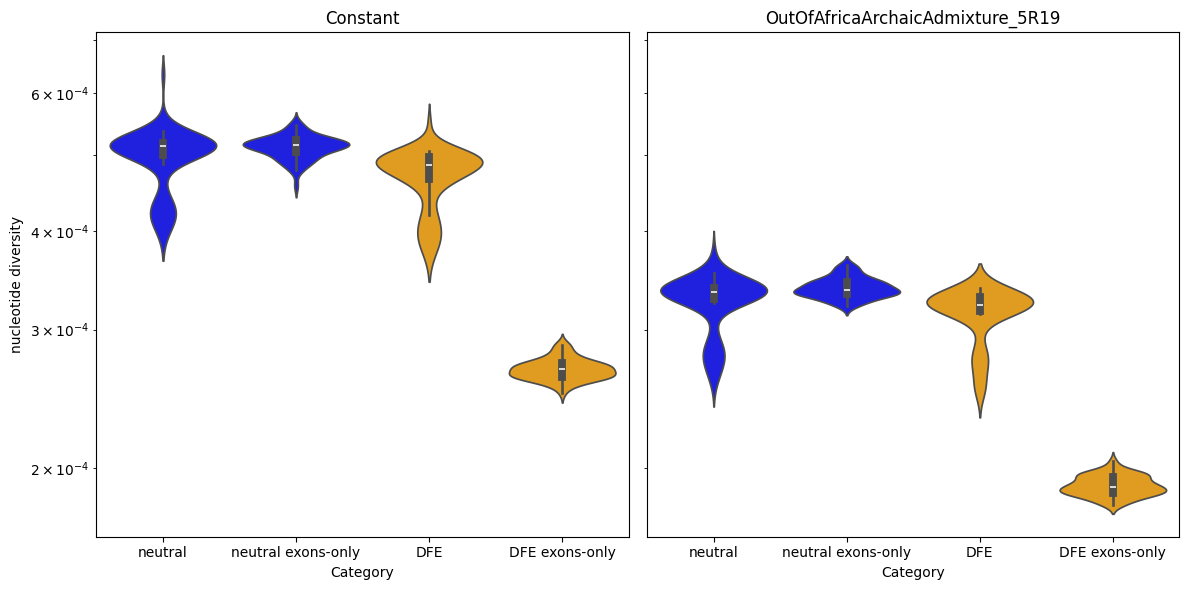
\includegraphics[width=\textwidth]{figures/HomSap/summary_stats.png}
    \caption{
    \label{fig:homsap-summary-stats}
    Genetic diversity in human simulations.
    Nucleotide diversity ($\pi$) was calculated for genomes simulated
    under constant population size (left panel) and under the out-of-Africa demographic model (right panel).
    Each panel shows four violin plots representing the distribution of $\pi$
    in genomes simulated without selection (blue) and genomes simulated with background selection (orange),
    calculated from either the entire genome (labeled neutral or DFE),
    or from exonic regions only (labeled exons-only).
    Each violin plot summarizes three replicate simulations generated under the relevant scenario.
    }
\end{figure}

\begin{figure}[h]
    \centering
    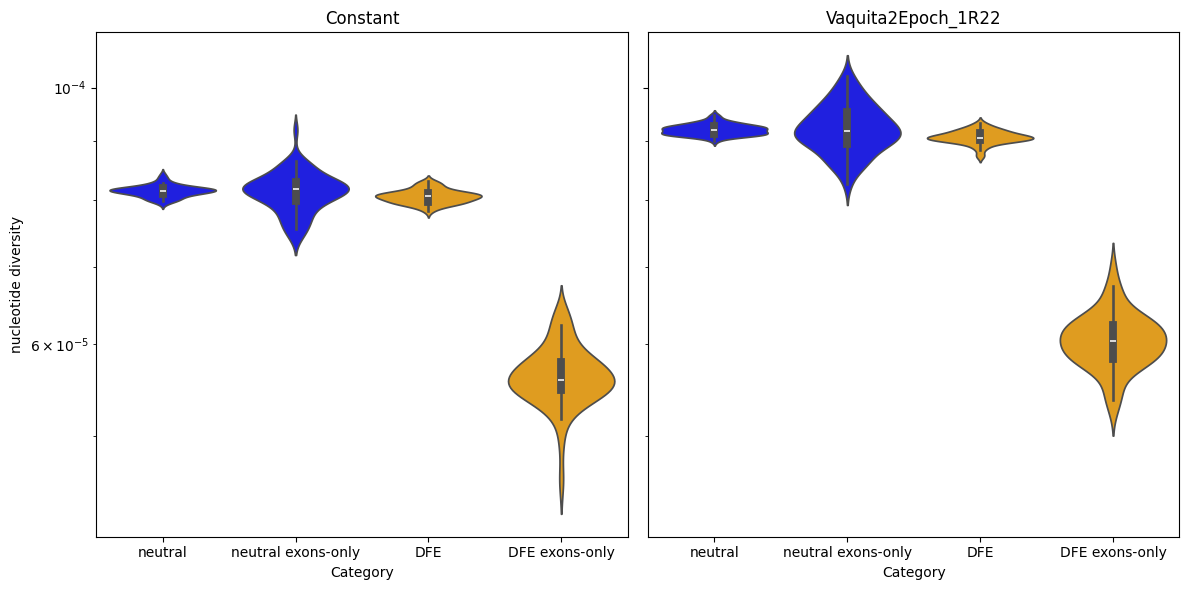
\includegraphics[width=\textwidth]{figures/PhoSin/summary_stats.png}
    \caption{
    \label{fig:vaquita-summary-stats}
    Genetic diversity in vaquita simulations.
    Nucleotide diversity ($\pi$) was calculated for genomes simulated
    under constant population size (left panel) and under the two-epoch demographic model (right panel).
    Each panel shows four violin plots representing the distribution of $\pi$
    in genomes simulated without selection (blue) and genomes simulated with background selection (orange),
    calculated from either the entire genome (labeled neutral or DFE),
    or from exonic regions only (labeled exons-only).
    Each violin plot summarizes three replicate simulations generated under the relevant scenario.
     }
\end{figure}

\begin{figure}[h]
    \centering
    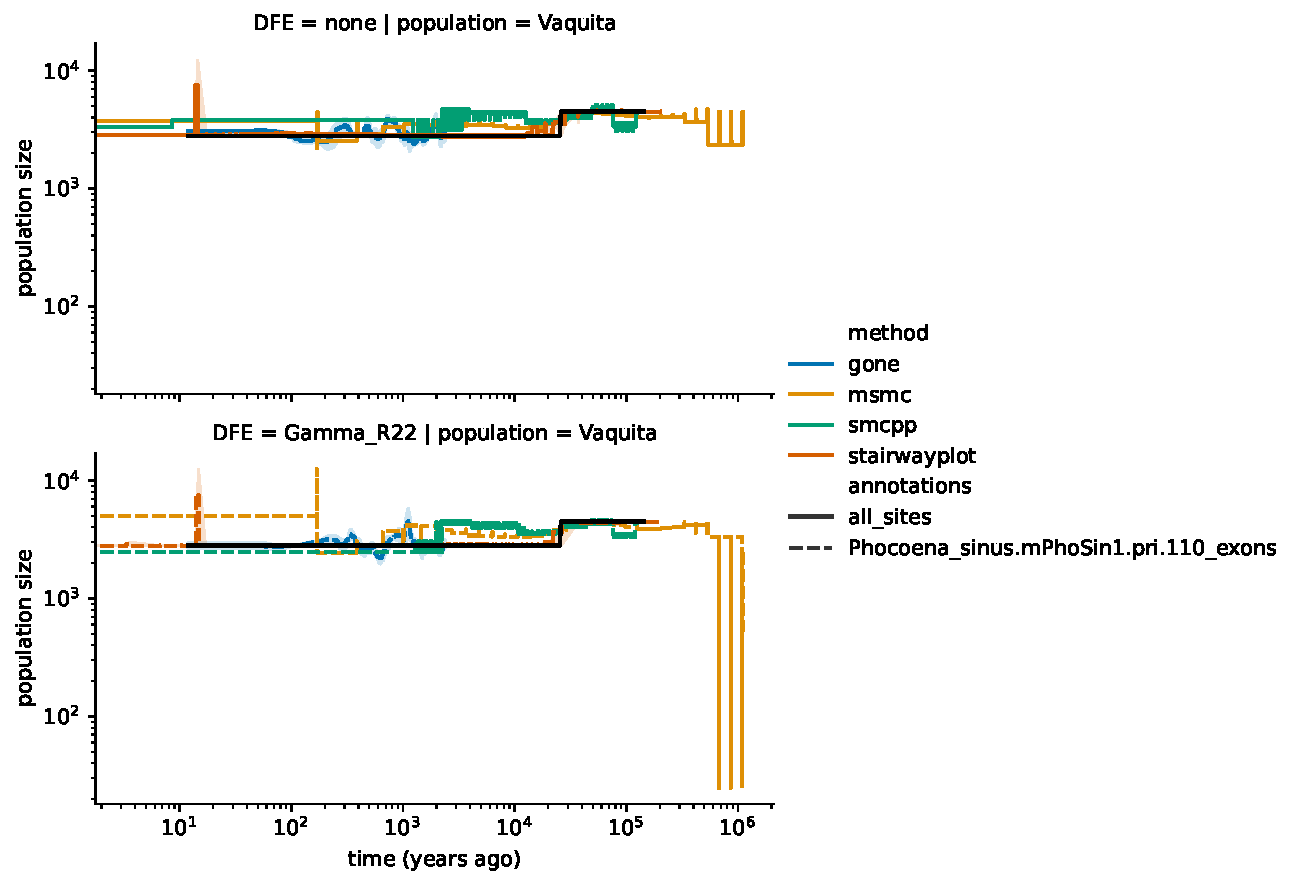
\includegraphics[width=\textwidth]{figures/PhoSin/Vaquita2Epoch_1R22/estimated_Ne_t_final.pdf}
    \caption{
    \label{fig:vaquita-demography}
    Inference of $N_e(t)$ from vaquita porpoise genomes simulated under a single population
    model of declining population size with and without purifying selection on exons.
    Inference is conducted using four methods: \stairway, \msmc, \smcpp and \gone.
    Each plot depicts the inferred $N_e(t)$ on the three datasets simulated without selection (blue)
    and the three datasets simulated with the background effects of purifying selection on exons (orange),
    alongside the true values of $N_e$ used in simulation (black).
}
\end{figure}


% constant size DFE figure
\begin{figure}[h]
    \centering
    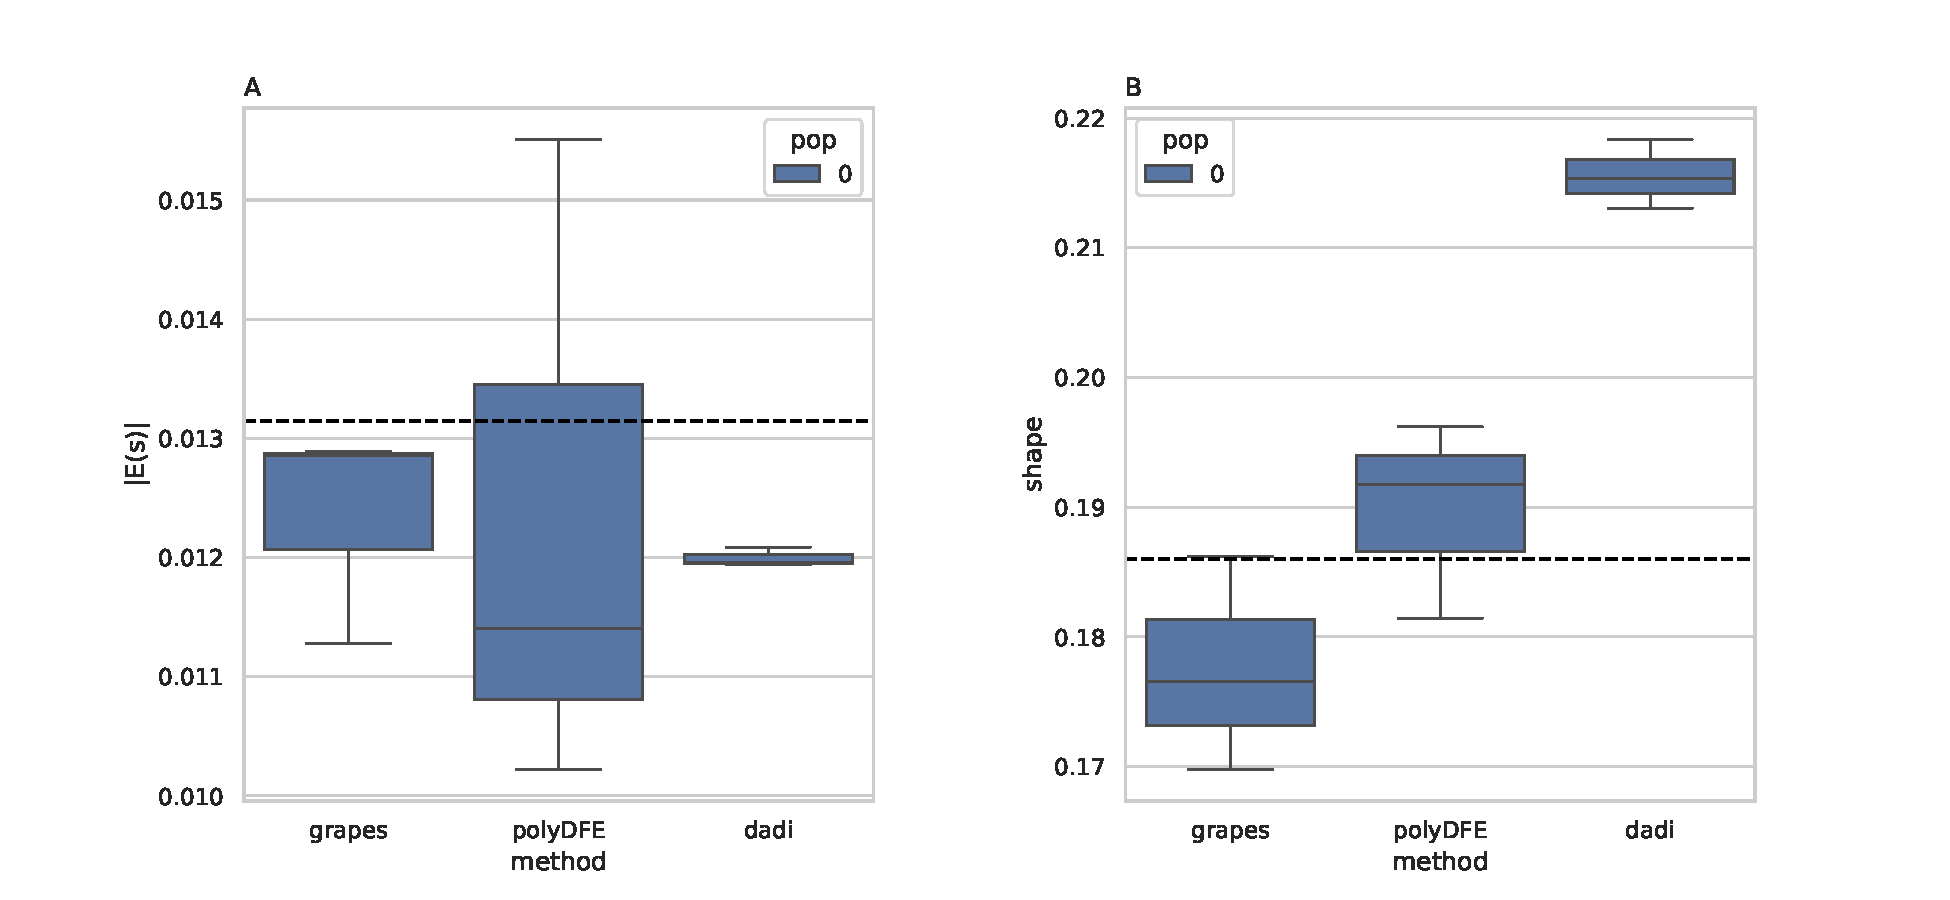
\includegraphics[width=\textwidth]{figures/HomSap/Constant/HomSap_Constant_Gamma_K17_ensembl_havana_104_exons_DFE_plot}
    \caption{
       Inferred versus simulated DFEs from human genomes simulated with
       a simple demographic model with one population with a constant size of $10,000$
       and a gamma-distributed DFE acting on exons (see \textbf{Methods}).
        DFE is inferred by three different methods: \grapes, \polydfe , and \dadicli.
        Mean absolute value of selection coefficient ($\lvert E(s) \rvert$, panel A) and shape parameter (panel B)
        are shown for each DFE inferred from all three simulated datasets
        with median values marked by horizontal bars
        and simulated values represented by dashed horizontal lines.
    }
    \label{fig:homsap-dfe.constant}
\end{figure}

\begin{figure}[h]
    \centering
    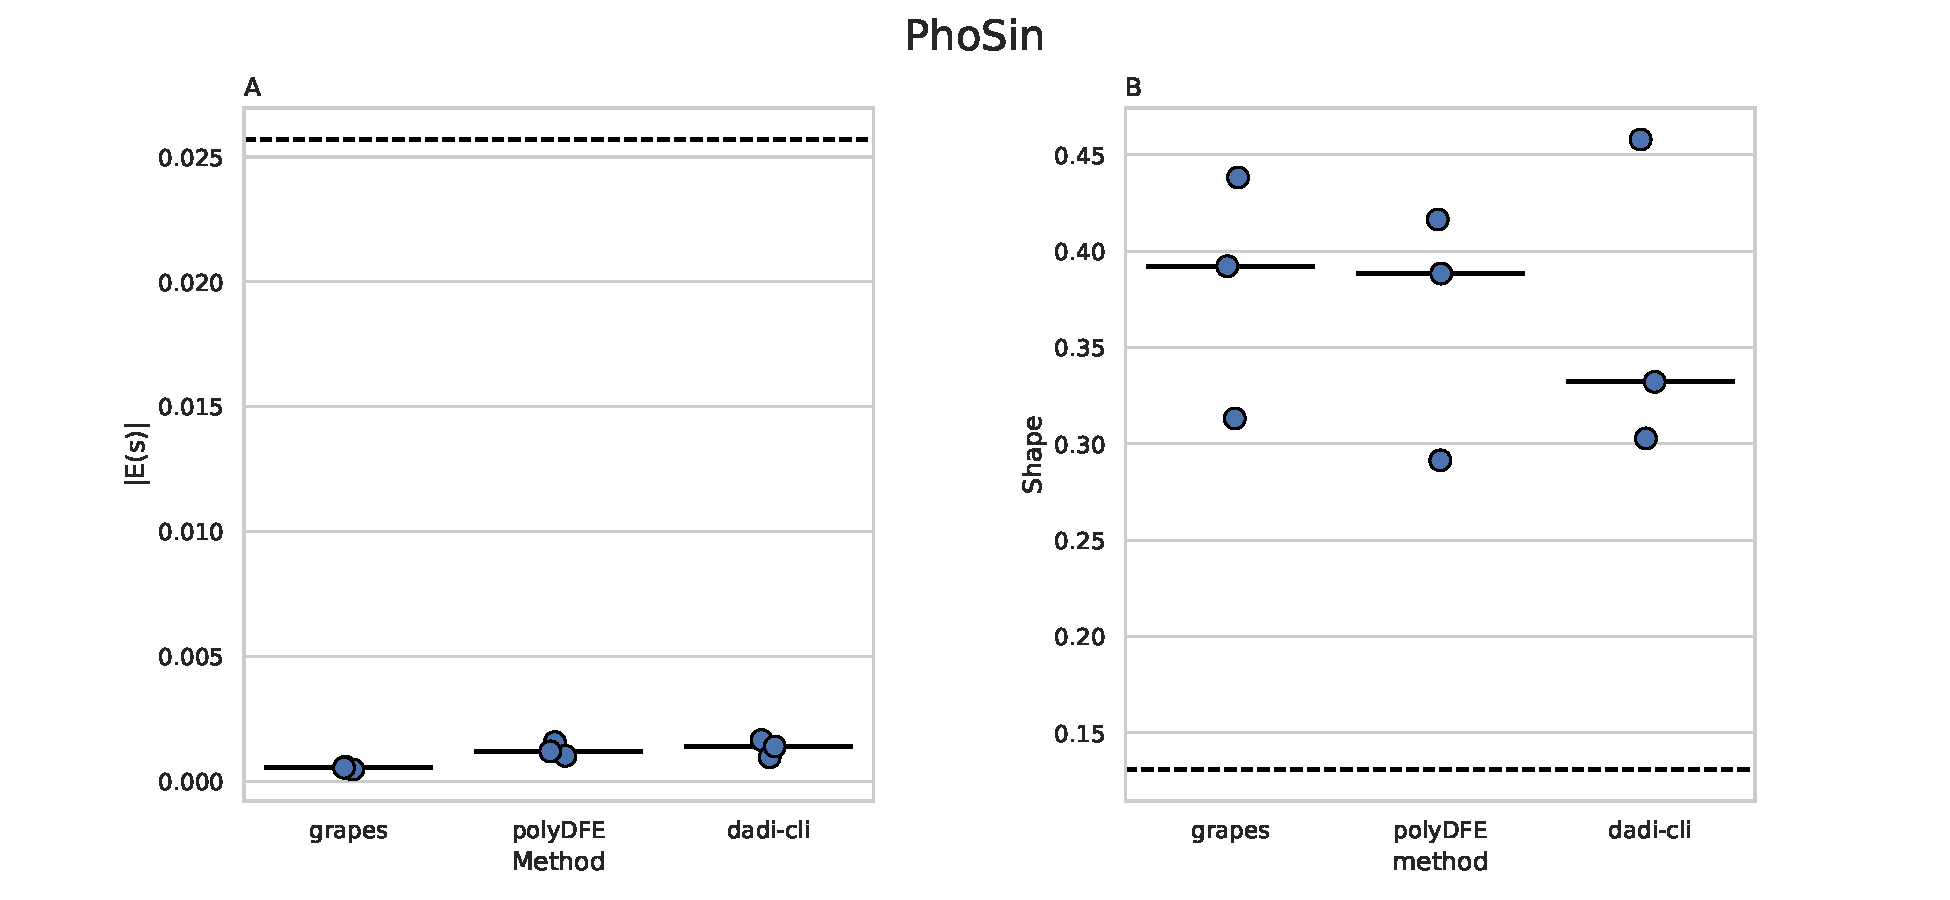
\includegraphics[width=\textwidth]{figures/PhoSin/Constant/PhoSin_Constant_Gamma_R22_Phocoena_sinus.mPhoSin1.pri.110_exons_DFE_plot.pdf}
    \caption{
    \label{fig:vaquita-dfe.constant}
        Inferred versus simulated DFEs from vaquita genomes simulated with
        a simple demographic model with one population with a constant size of $3,500$
        and a gamma-distributed DFE acting on exons
        with a relationship between the selection coefficient ($s$) and dominance coefficient ($h$) (see \textbf{Methods}).
        DFE is inferred by three different methods: \grapes, \polydfe , and \dadicli.
        Mean absolute value of selection coefficient ($\lvert E(s) \rvert$, panel A) and shape parameter (panel B)
        are shown for each DFE inferred from all three simulated datasets
        with median values marked by horizontal bars
        and simulated values represented by dashed horizontal lines.
    }
\end{figure}

%IG: this fig is not cited anywhere and does not appear to provide crucial insights
%\begin{figure}[h]
%    \centering
%    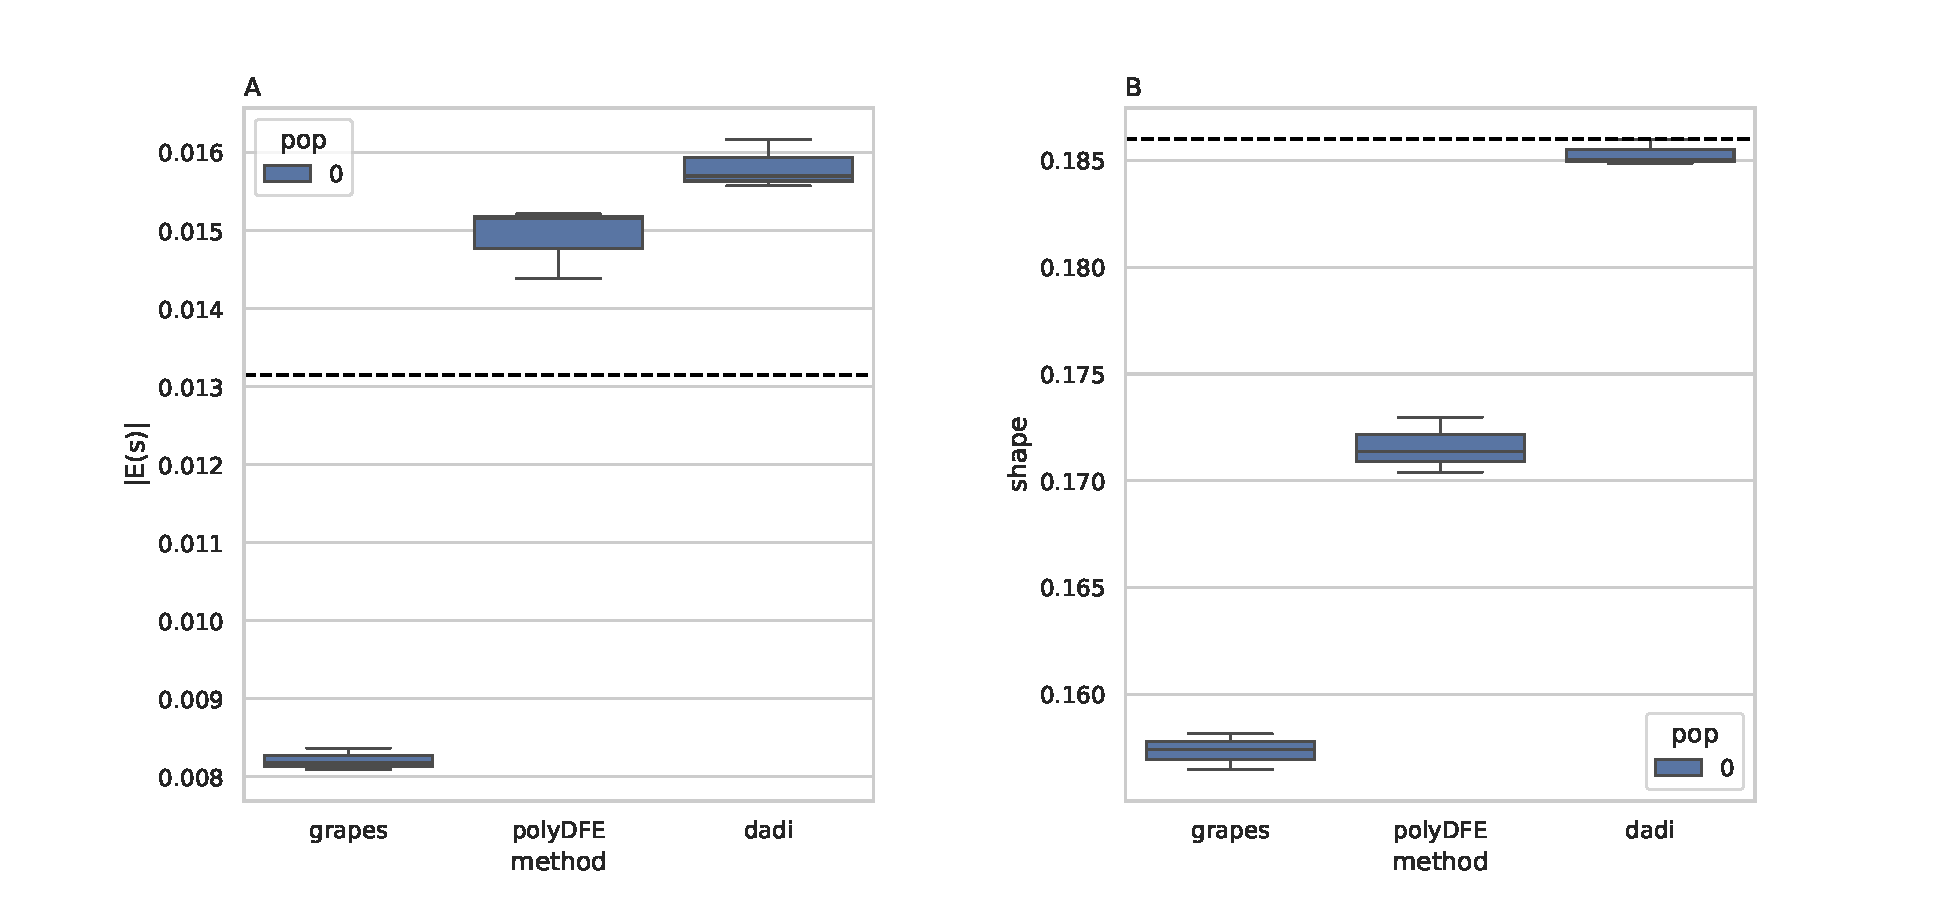
\includegraphics[width=\textwidth]{figures/HomSap/Constant/HomSap_Constant_Gamma_K17_all_sites_DFE_plot}
%    \caption{
%    \label{fig:homsap-dfe.constant.all_sites}
%    Performance of methods to infer the distribution of fitness effects (DFE) from genetic data
%    under constant population size  where all sites along the simulated chromosome can experience selected and neutral mutation
%    as opposed to exonic regions only.\\
%    }
%\end{figure}



% roc curves for sweeps
\begin{figure}[h]
    \centering
    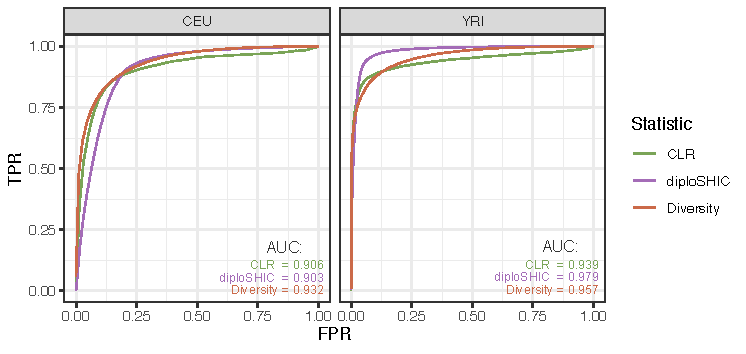
\includegraphics[width=0.8 \textwidth]{figures/sweeps/roc_neutral_null.pdf}
    \caption{
    \label{fig:roc-curves}
    Receiver operating characteristic (ROC) curves for the three methods for detecting sweeps:
    \sweepfinder (labeled CLR), \diploshic, and reduced diversity ($\pi$).
    True positive rates (TPR) were computed across all datasets simulated with selective sweeps,
    and false positive rates (FPR) were established by applying the methods to genomes simulated
    under the same settings but without sweeps (the BGS model; see \textbf{Methods}).
    Area under the curve (AUC) scores are shown for each method.
    }
\end{figure}


%sweep power vs exon density
\begin{figure}[h]
    \centering
    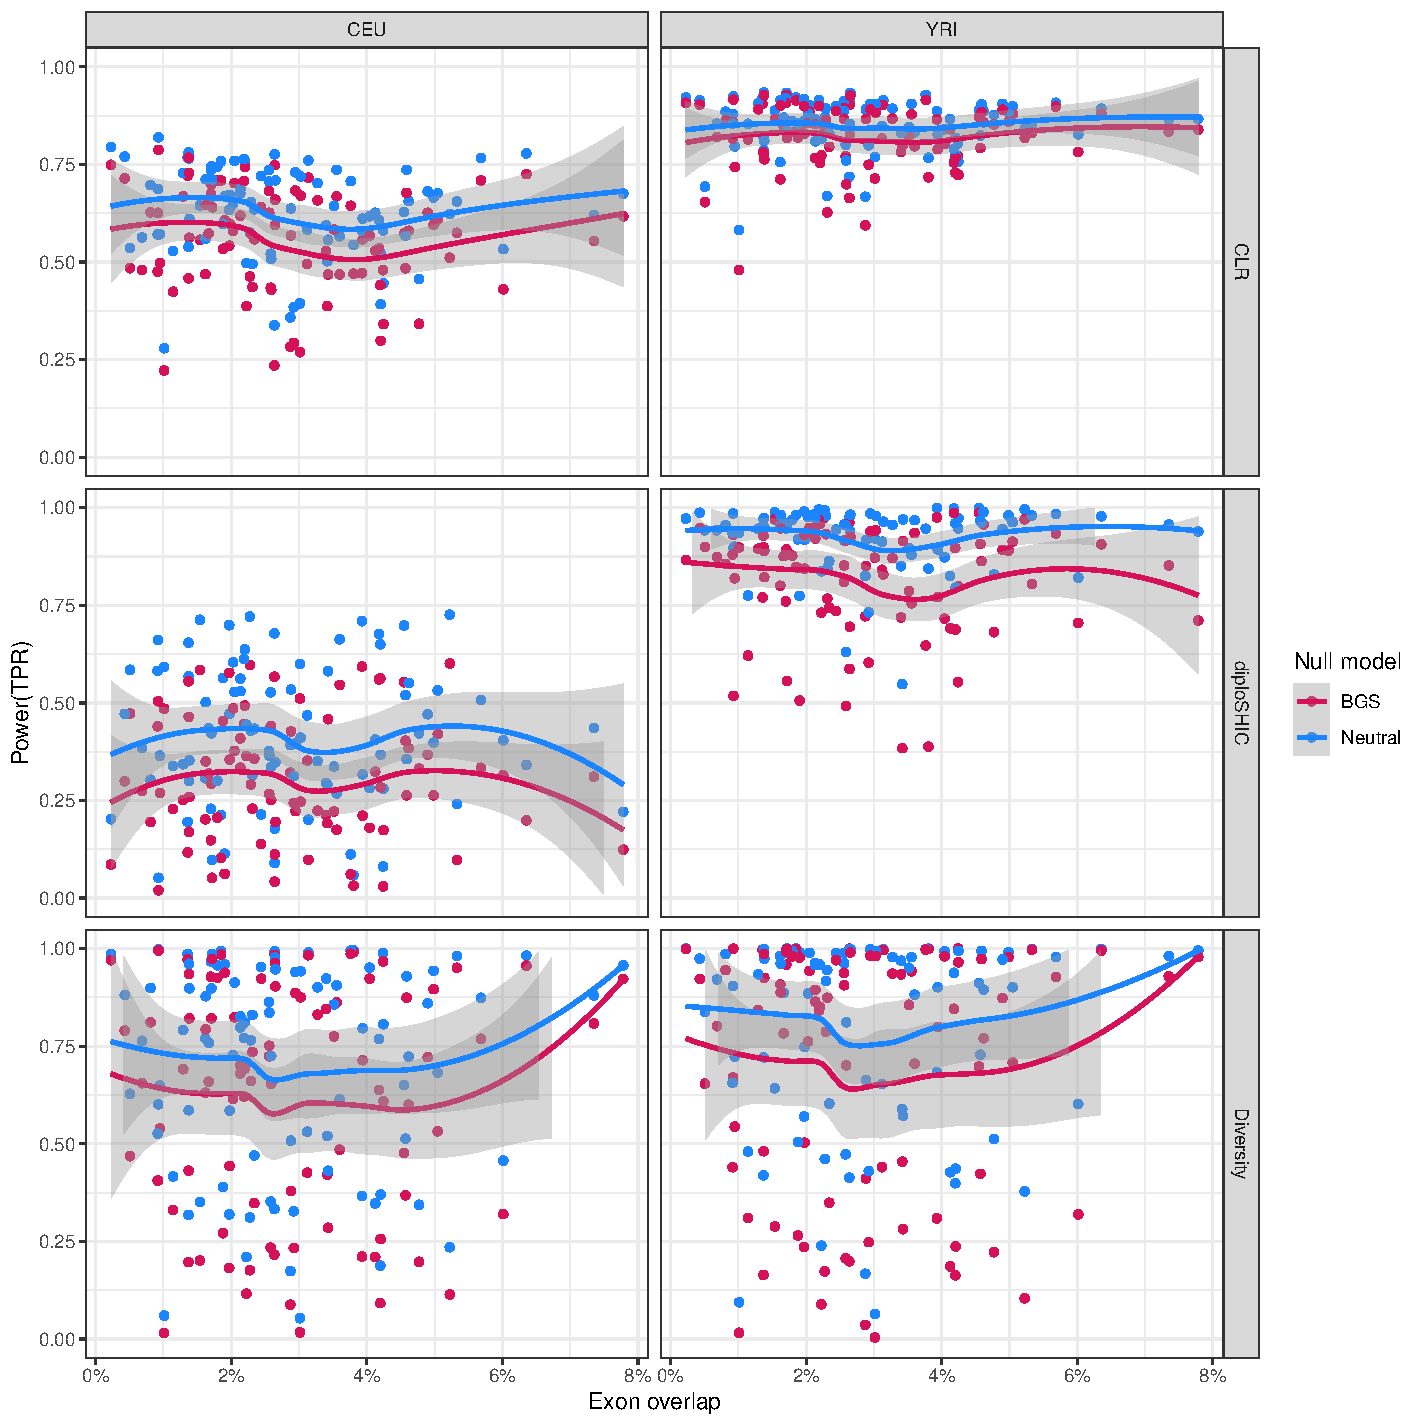
\includegraphics[width=0.8 \textwidth]{figures/sweeps/relationship_power_exon.pdf}
    \caption{
        Power to detect selective sweeps
        as a function of local exon density.
        This figure shows the same power estimates shown in Figure \ref{fig:chr1_power},
        but with the genomic segments plotted against their
        exon density (percentage of exonic bases per window) instead of position along chromosome 1.
    	Genomic segments were simulated with sweeps under a three population out-of-Africa model
        and with background selection from deleterious mutations in exons.
        Three methods for detecting sweeps were applied to simulated data:
        \sweepfinder (top row-- labeled CLR),
        \diploshic (middle row),
        and reduced diversity ($\pi$) (bottom row).
        Power (true positive rate) is shown for these methods for the CEU and YRI
        samples (left and right respectively).
        The thresholds of the test statistics were set to obtain a
        $5\%$ false positive rate under a neutral null model (blue)
        and a null model with background selection from deleterious mutations in exons (red).
        Fitted lines represent loess smoothed regressions.
    }
    \label{fig:power-exon}
\end{figure}

\stopsupplement
\end{document}
